\documentclass[conference]{IEEEtran}

\usepackage{graphicx}
\usepackage{amsthm}
\usepackage{amssymb}
\usepackage{amsmath}
\usepackage{algorithm}
\usepackage{algorithmicx}
\usepackage{algpseudocode}
\usepackage{booktabs}
\usepackage{color}
%\usepackage{epstopdf}

\renewcommand{\baselinestretch}{0.98}
\setlength{\textfloatsep}{10pt}
\setlength{\abovecaptionskip}{10pt}

\newtheorem{definition}{Definition}
\theoremstyle{definition}
\newtheorem{theorem}{Theorem}
%\theoremstyle{plain}
\newtheorem{lemma}{Lemma}
%\theoremstyle{plain}
\newtheorem{proposition}{Proposition}
%\theoremstyle{plain}
\newtheorem{corollary}{Corollary}
%\theoremstyle{plain}

\begin{document}

\title{On Designing Collusion-Resistant Incentive Mechanisms for Mobile Crowdsensing Systems}
\author{
%Shiyu Ji\textsuperscript\textdagger, Tingting Chen\textsuperscript\textsection\\
%\textdagger\hspace{0.1cm}Oklahoma State University, shiyu@cs.okstate.edu\\
%\textsection\hspace{0.1cm}California State Polytechnic University, Pomona, tingtingchen@csupomona.edu
}
\maketitle

{\color{black}
\begin{abstract}
%With the rise of smartphones, crowdsensing applications have tremendously increasing trending. As a result, many incentive and privacy issues are worth researching. This paper gives detailed discussions on collusion resistant incentive mechanisms for crowdsensing applications. We analyze the continuous crowdsensing game in which users take sensing time to finish tasks and get payment. Two fundamental criteria are found: one is to judge whether a truthful incentive mechanism can resist any collusion without profit trading by achieving group strategyproof equilibrium, and the other is to judge whether a truthful mechanism can defend against any collusion even with profit trading by achieving n-truthful equilibrium. We also propose a concrete solution that not only satisfies both the criteria, but also maximizes the platform utility. However, sometimes users can only finish the sensing in discretized units and thus the continuous sensing time assumption may not hold any more. To address this discrete scenario, we give detailed analysis and propose a heuristic incentive solution that not only resists any collusion attack, but also preserves differential privacy of the participatory users. Extensive simulations verify our results. To the best of our knowledge, we are the first to investigate the collusion resistant incentive mechanisms for crowdsensing applications.

With the rise of smartphones, crowdsensing applications have tremendously increasing trending. As a result, many incentive issues are worth researching. In this paper, we give detailed discussions on collusion resistant incentive mechanisms for crowdsensing applications. Two fundamental criteria are found: one is to judge whether a truthful incentive mechanism can resist any collusion without profit trading by achieving group strategyproof equilibrium, and the other is to judge whether a truthful mechanism can defend against any collusion even with 
profit trading by achieving t-truthful equilibrium. Furthermore, we also propose our solution which can resist any form of collusion attack, even including profit trading among the attackers. Extensive simulations verify our results. To the best of our knowledge, we are the first to investigate the collusion resistant incentive mechanisms for crowdsensing applications.
\end{abstract}
}

\section{Introduction}
With the rapidly increasing use of portable devices (e.g. smartphones), there are plenty of research works \cite{ganti2011mobile, vukovic2010ubiquitous, cortes2002coverage} and numerous applications \cite{nawaz2013parksense, rai2012zee, yan2011crowdpark, kazman2009metropolis} on mobile sensing. Sensing apps on smartphones allow people to sense and collect different kinds of information ubiquitously. 
To sufficiently explore the sensing capability of each sensor within the network, crowdsensing \cite{howe2006rise} \cite{ganti2011mobile} techniques can be applied. For instance, by using the  crowdsensing platform, we can access the up-to-date parking slots information on the neighboring community \cite{nawaz2013parksense, yan2011crowdpark}, or monitor weather changes \cite{kazman2009metropolis}.

The incentive issues in crowdsensing systems have been extensively studied \cite{yang2012crowdsourcing, zhang2012reputation, koutsopoulos2013optimal, singla2013truthful, jaimes2012location}. Crowdsensing work embodies costs in nature (e.g. service fees, battery usage, etc). Hence we need to stimulate the participating users to contribute their sensed data,  by giving them some incentives (e.g., in monetary forms) to cover the cost incurred by individual sensing activities. Existing incentive mechanisms (e.g., \cite{yang2012crowdsourcing, zhang2012reputation, jaimes2012location}) use game theoretical approaches to achieve different equilibria. For instance, strategyproof crowdsensing incentive mechanisms\cite{moulin2001strategyproof, chen2013sparc, feng2013imac} can guarantee that it is to the best interest of each participating user to honestly report their information such as sensing cost. However, strategyproofness cannot eliminate the possibility that a group of users collaborate to cheat in the system and harm the system or other users' utility. 
Unfortunately, there has not been any existing work that systematically investigates the collusion attack problem in crowdsensing incentive mechanisms.
%These mechanisms usually need to know some information about each user (i.e. sensing cost and revenue). However, for many cases we cannot guarantee the participatory users are always honest. In other words, some users may give false reports deceitfully. Hence strategyproofness (or truthfulness) arises to eliminate these cheatings . Strategyproof incentive mechanism is safe to use for any participatory user, assuming the users are \emph{selfish} and never trust each other completely. This implies strategyproofness is not strong enough to defend against collusion attack, in which group of users have complete trust between each other.

%How to resist collusion in crowdsensing incentive mechanisms is an important open problem,

In real-world crowdsensing applications, a single entity may simultaneously own a number of mobile devices, e.g. smartphones, laptops, tablets, watches, etc. These devices may have diverse sensing costs and but can participate the same crowdsensing task. In the crowdsensing procedure, since the payment that each user receives is usually correlated to its sensing contribution and the involved cost, the same owner can manipulate a group of devices' sensing strategies at the same time and make them collaboratively cheat (e.g., reporting carefully-calculated fake cost information to rule out other potential participants) for better payoffs as a collusion. It creates serious problems for the platform, such as losing system-wide utility and deteriorating other users' enthusiasm to participate.
%Many existing crowdsensing incentive mechanisms \cite{yang2012crowdsourcing,koutsopoulos2013optimal,zheng2014strategy} that assume individual rationality cannot .

Collusion attack is an important but difficult problem to address in general \cite{zhong2007designing, wang2006low, jurca2007collusion}. 
The difficulty lies in two aspects: \textbf{1)} A variety of collusion strategies (e.g., with or without profit trading) make the mitigation challenging. It means that in practice it requires security expertise to consider as many collusion scenarios as possible for a specific setting and provide technical solutions to mitigate the known collusion attacks. But like other penetration analysis, there is no guarantee of guard against unexamined cases. \textbf{2)} Difficulty exists when trying to provide theoretical guarantee of guard in the incentive mechanism design. 
As we mentioned earlier, since only strategyproofness cannot provide collusion resistance \cite{zhong2007designing}, people try to use other game theoretical solution concepts such as \emph{Group Strategyproof Equilibrium} \cite{jain1999group} to achieve collusion resistance. %So far  is one of the standard collusion resistant solutions that can give truthful mechanisms.
However, within the scope of wireless networks, sometimes it is not possible at all to achieve any group strategyproof equilibrium in some games. For example, one can never achieve any group strategyproofness in theory for noncooperative routing games in wireless ad hoc networks \cite{zhong2007designing}. When the possibility that colluding nodes can trade profit among them, this problem becomes even harder. For the same routing problem, we cannot obtain any strategyproofness if the colluding users can trade profit among them \cite{wang2006low}.

%For the crowdsensing problem that we focus on in this paper, it is unknown yet whether it is theoretically possible to achieve group-strategyproofness through our incentive mechanism design. 

In this paper we systematically study the collusion-resistance problem in crowdsensing incentive mechanism design. Our goals are not only to provide theoretical results, for example, on the possibility of achieving group strategyproofness, but also to make the theoretical results have direct benefits in practice. In particular, we notice that even with the formal definition of group-strategyproofness and \textit{t-truthfulness} (defense against profit trading), it is very challenging for mobile crowdsensing practitioners to map the theoretical definitions to their concrete systems that they have or are about to design. In this paper, we will provide much more straightforward criteria/techniques to judge whether a given incentive mechanism is group-strategyproof or t-truthful, so that the designer or practitioners can easily apply. This effort has significant benefits in reducing unnecessary overhead and meanwhile maintains the security guarantee. For instance, if we can easily determine that the incentive mechanism can intrinsically defend against profit trading by achieving t-truthfulness, then we do not have to use extra cryptographic protocols such as Designated Verifier Signatures \cite{jakobsson1996designated} or Restricted Verifier Signatures \cite{zhong2007designing} that are used to restrict profit trading. Thus the computation and communication overhead are reduced.

%We not only provide solutions to the above question but seek answers to practical ones such as 

%Although these facts give pessimistic messages, they cannot rule out the possibility that we may achieve group strategyproofness for crowdsensing games. 
%The question ``For crowdsensing game, is it possible to propose a t-truthful incentive mechanism \cite{goldberg2005collusion} which is strong enough to resist collusion with profit trading?'' %and ``Is it doable to give an extremely strong incentive mechanism, which not only defends against collusions, but also preserves the privacy of participatory users?'' 
%still remains unanswered. To the best of our knowledge, these possibilities have not been fully investigated by most existing literatures. Hence this paper tries to fill this void.

Our major contributions are summarized as follows:

\newcount\itemcount
\itemcount 1\relax
\def\bolditem{\par{\bf(\the\itemcount)}\enspace\advance\itemcount 1\relax}

\bolditem We investigate a popular type of crowdsensing games, in which each contributing user takes some sensing time to finish the assigned tasks and earns the promised payment from the platform. We not only find it is feasible to design group strategyproof incentive mechanisms for this type of crowdsensing game, but also obtain the straightforward criteria to judge whether a given strategy-proof incentive mechanism can achieve group strategyproofness. Moreover, we rigorously derive the criteria to judge whether a truthful mechanism is t-truthful to guard against profit trading. %In other words, we show that it is theoretically possible to resist any collusion attack, even with profit trading, for the crowdsensing game. 
%By correctly judging whether an incentive mechanism can resist collusion or profit trading, we can gain many benefits in the real world. For example, \cite{archer2004approximation} has given the truthful incentive mechanism that can successfully defend against collusion in multicast cost sharing by achieving group strategyproofness. If each user cannot trust others completely, the information from the users can be reliable and the system does not have to use extra protocols to ensure no one is cheating. In this light, we can obtain reliable information and save communication overhead if we can show the truthful incentive mechanism can achieve group strategyproofness. %For the scenario of wireless ad hoc routing, \cite{zhong2007designing} has given the collusion resistant incentive mechanism that cannot achieve n-truthfulness. That is, their proposed incentive mechanism cannot solely eliminate the possibility of profit trading. This implies that one has to take additional actions to rigorously defend against profit trading, for example, by leveraging some public cryptographic protocols such as Designated Verifier Signatures \cite{jakobsson1996designated} or Restricted Verifier Signatures \cite{zhong2007designing}. In other words, if we can show the incentive mechanism can intrinsically defend against profit trading by achieving n-truthfulness, then we do not have to use the extra cryptographic protocols and hence reduce the computation and communication overhead. Hence our obtained criteria can give practical benefits.} %Furthermore, based on both the obtained criteria, we propose a concrete incentive mechanism which is not only collusion resistant, but also maximizes the platform utility.

\bolditem For another group of typical crowdsensing game, in which each contributing user finishes the assigned discrete sensing tasks to earn corresponding payment, we propose a concrete collusion-resistant incentive mechanism. %Sensing tasks are assigned by the crowdsensing platform based on the claimed cost of each user. 
%We propose an  to the discrete crowdsensing game. 
%(WE NEED TO EXPLAIN THE DIFFICULTY FOR DISCRETE MODEL, ESPECIALLY THE CHALLENGE WE FACE WHEN DEFENDING AGAINST PROFIT TRADING, WHICH IS DIFFERENT FROM CONTINUOUS MODEL.)
{\color{black}Differently from the case in which the sensing time can take any positive value, assigning discrete sensing tasks may let each user not have to be completely truthful, since usually a small perturbation on truthful strategy will not change the user utility. Hence it can be more difficult to establish a truthful incentive mechanism that can resist collusion, or even profit trading among the colluding nodes. 
However, we can show that our incentive mechanism can achieve group strategyproofness and t-truthfulness. In other words, our solution can defend against colluded cheating, even with profit trading.}

%\bolditem {\color{black}Privacy issues in crowdsensing have attracted extensive researchers' attention \cite{agarwal2013protectmyprivacy, varshney2012privacy}. We take the threat model in which the attacker may know the number of assigned tasks to each user by traffic analysis or timing attacks. While assuming the sensing cost and the identity of each user should be private, we propose a new discrete incentive mechanism, and rigorously show that this proposed mechanism not only can achieve group strategyproofness and n-truthfulness, but also can preserve 0-differential privacy.} Hence our proposed mechanism for discrete incentives not only can resist any collusion (even with profit trading), but also can well preserve the users' privacy.

\bolditem To verify our theoretic results, we also perform extensive simulations, and we show that all the experimental results support our findings.

{\color{black}
The remainder of this paper is organized as follows. Section \ref{sec:TP} gives the necessary technical preliminaries including equilibria, collusion attack and profit trading. Section \ref{sec:PFSM} discusses the basic settings of the crowdsensing game model. Section \ref{sec:GSIM} gives the criteria whether a truthful crowdsensing incentive mechanism can be group strategyproof. Section \ref{sec:DFPT} gives the criteria whether a truthful mechanism can be t-truthful. 
In Section \ref{sec:discrete} we propose the discrete collusion resistant incentive mechanism which can achieve both group strategyproofness and t-truthfulness. 
%In Section \ref{sec:pr} we propose our discrete crowdsensing incentive mechanism, which not only can defend against collusion attacks, even including profit trading, but also can well preserve users' identity privacy. 
Section \ref{sec:sim} gives the simulation results and Section \ref{sec:rw} summarizes the related literatures. Section \ref{sec:con} concludes this paper.
}

%The remainder of this paper is organized as follows. Section \ref{sec:TP} gives the necessary technical preliminaries including equilibria, collusion attack, profit trading and differential privacy. Section \ref{sec:PFSM} discusses the basic settings of the crowdsensing game model. Section \ref{sec:GSIM} gives the criteria whether a truthful crowdsensing incentive mechanism can be group strategyproof. Section \ref{sec:DFPT} gives the criteria whether a truthful mechanism can be n-truthful. Section \ref{sec:opu} proposes our concrete continuous collusion resistant incentive mechanism that can also maximize the platform utility. In Section \ref{sec:discrete} we propose the discrete collusion resistant incentive mechanism, and then give discussions on the incentive and privacy issues on the discrete crowdsensing game. We also propose our heuristic solutions to eliminate some singular privacy leakage cases. Section \ref{sec:sim} gives the simulation results and Section \ref{sec:rw} summarizes the related literatures. Section \ref{sec:con} concludes this paper.

%The remainder of this paper is organized as follows. Section \ref{sec:TP} gives the necessary technical preliminaries including equilibria, collusion attack, profit trading and differential privacy. Section \ref{sec:PFSM} discusses the basic settings of the general crowdsensing game model. In Section \ref{sec:discrete} we propose the discrete collusion resistant incentive mechanism, and then give discussions on the incentive and privacy issues on the discrete crowdsensing game. We also propose our heuristic solutions to eliminate some singular privacy leakage cases. Section \ref{sec:sim} gives the simulation results and Section \ref{sec:rw} summarizes the related literatures. Section \ref{sec:con} concludes this paper.

\section{Technical Preliminaries}
\label{sec:TP}
This section describes the technical preliminaries including the basics of crowdsensing game, the concept of equilibrium in game theory, and the idea of profit trading. We also give some useful local properties of bivariate functions in the appendix. Table \ref{tab:symbol_list} presents the frequently used symbols in this paper.\footnotetext[1]{Similarly, by removing subscripts, $t$ denotes the sensing time profile, $p$ denotes the payment profile, $u$ denotes the user utility profile, $n$ denotes the profile of number of tasks, etc.}
\begin{table}[!t]
\begin{tabular}{l l}
\toprule
Notation & Description\\
\hline
$U$ & the set of users\\
$n$ & the number of users: $|U|$ \\
%$R$ & the baseline gain of the platform\\
$s_i$ & the claimed cost unit (strategy) of user $i$\\
$s$ & the strategy profile of all users \footnotemark[1]\\
$s_{-i}$ & the strategy profile excluding user $i$'s strategy\\
$\kappa_i$ & the cost unit of user $i$\\
$p_i$ & the (promised) payment to user $i$\\
$t_i$ & the required sensing time of user $i$\\
$u_i$ & the utility function of user $i$\\
$u_p$ & the utility function of the platform\\
$n_i$ & number of the assigned tasks to user $i$\\
$m$	& number of partitions\\
$d$ & partition length\\
$f(x, y_0)$ & the slice function of $f(x,y)$ by fixing $y = y_0$\\
$B$ & budget, upper bound of the payment sum $\sum p_i$\\
$R$ & the number of remaining sensing tasks to do\\
\bottomrule
\smallskip
\end{tabular}
\caption{Frequently used notations}
\label{tab:symbol_list}
\end{table}
\addtocounter{footnote}{1}

\subsection{Crowdsensing Game}
\label{subsec:CG}
{
We introduce the general game model of crowdsensing system, which is used in the majority of existing literatures \cite{yang2012crowdsourcing,koutsopoulos2013optimal,luo2014profit,zhang2014free,liu2014social,yan2015ifc}. The crowdsensing system consists of $n$ participating users, who are all the users \emph{willing} to contribute in the crowdsensing work (e.g. smartphones, mobile sensors) and one crowdsensing platform (e.g. BOINC \cite{anderson2004boinc}). The $n$ users voluntarily participate in crowdsensing and contribute their sensing results. The platform aggregates the sensing results from the $n$ users and maintains the crowdsensing system. %For each contributing user\footnote{contributing users are the users who \emph{actually} participate in the crowdsensing by \emph{contributing} sensing work.}, sensing work incurs cost in monetary form, such as battery charge and communication fees. 
To compensate the users' sensing costs and stimulate their participation, the platform distributes some payment to each user as the reward. The payment is determined by each user's strategy (i.e., its claimed sensing cost). Denote by $c_i$ the sensing cost of user $i$, and let $p_i$ be the promised payment from the platform to user $i$. If user $i$ can complete the sensing task as promised, then the utility of user $i$ is
\begin{equation}
\label{eqn:user_utility_1}
u_i = p_i-c_i.
\end{equation}
%Here the utility is the incentive for each user to participate in crowdsensing. 
Due to individual rationality, each user wants to maximize its own utility. %To address the incentive issues, we need an incentive mechanism, which is an interactive scheme between the users and the platform to determine the payment to each user.

{\color{blue}
For the platform, we may consider the budget feasibility for many practical scenarios \cite{zhao2014crowdsource,singer2013pricing,singla2013truthful}. That is, the total sum of the payments $p_i$ must be no more than some budget $B$. In this paper, we will show that the payment sum of our proposed mechanisms can be upper bounded.
}
%We next analyze the platform utility. {Based on the ideas of \cite{yang2012crowdsourcing,luo2014profit,zhang2014free,liu2014social}}, the platform utility has a diminishing return on the contribution of each user. \cite{yan2015ifc} gives the idea to calculate the contributed gain from all the contributing users by summation over $U$. That is, we have its closed-form as following:
%\begin{equation}
%\label{eqn:plat_utility}
%u_p=\sum_{i\in U}\lambda_i\log (1+t_i)-p_i.
%\end{equation}
%%Here $R$ is the baseline reward (i.e. the fixed reward as the crowdsensing finishes certain tasks).\footnote{In many existing models such as \cite{yang2012crowdsourcing}, there is no fixed baseline reward, and the gain primarily relies on the collected information. If so, $R=0$. If there are some external fundings provided by people who will use the collected information, then $R>0$.} {\color{black}As in Section \ref{sec:opu}, a positive baseline reward can well guarantee the participation of the platform, i.e. $R>0$.} $\lambda_i$ is a fixed parameter for each user $i$,\footnote{By assigning different $\lambda_i$, we can handle the scenarios that the platform treats the users with different weights. This generalizes the uniform weight assumption in some existing works, such as \cite{yang2012crowdsourcing,zhang2014free}.} and $t_i$ is the measurement of user $i$\rq{}s contribution (i.e. sensing time or sensed data). We must guarantee the platform utility $u_p>0$ so that our crowdsensing can keep working since it is making money.
%Here $\lambda_i$ is a fixed parameter for each user $i$,\footnote{By assigning different $\lambda_i$, we can handle the scenarios that the platform treats the users with different weights. This generalizes the uniform weight assumption in some existing literatures, such as \cite{yang2012crowdsourcing,zhang2014free}.} and $t_i$ is the measurement of user $i$\rq{}s contribution (i.e. sensing time or sensed data). We must guarantee the platform utility $u_p>0$ so that our crowdsensing can keep working.
}

\subsection{Collusion Attack and Group Strategyproof Equilibrium}

{\color{black}
The major objective of designing incentive mechanisms is to achieve a equilibrium, the state when each user has maximized its own utility and no user can increase its utility by unilaterally taking a different strategy. If one expects to eliminate the possibility that some users take actions deceitfully, a \emph{strategyproof} equilibrium is required. %Strategyproof equilibrium satisfies Incentive Compatibility (IC) and Individual Rationality (IR). IC says each user has to make actions truthfully (i.e., to report its sensing cost honestly) to maximize its utility, and IR says each user utility must be non-negative since any user can quit the game to avoid negative utility. 
Unfortunately, a strategyproof equilibrium is not strong enough to eliminate collusion among the users, since it is possible that some users \emph{collude} to alter their strategies simultaneously, in order to let some of them gain more utilities without decreasing any utility of theirs \cite{zhong2007designing}. 

%%To better understand this point, consider the following simple example. Vickrey--–Clarke--–Groves (VCG) auction \cite{vickrey1961counterspeculation} is a widely used strategyproof incentive mechanism. The basic idea of VCG can be summarized as: the highest bidder wins but is paid by the second highest, while assuming each user has no idea about the bids (sealed) or true costs of any other users. For example, there are only two users $A$ and $B$ in the game. There is only one sensing task, which can be done by exactly one of $A$ and $B$ individually. By completing the sensing task, $A$ can obtain 1 as revenue, and $B$ can get 2 as revenue. Each user is supposed to report its claimed revenue to the auction platform as its own strategy. Then the platform selects the highest bidder as winner and asks the winner to pay the charge, which is exactly the same as the bid of the other user. If $A$ claims 1 and $B$ claims 2, then we choose $B$ as winner and $B$ has to pay 1. Hence the utility of $B$ is $2-1=1$ and $A$ has utility of 0. It can be shown that this mechanism is strategyproof. That is, each user can always maximize its own utility by bidding its true revenue honestly, whatever the other bids. However, this solution cannot resist collusion attack, in which $A$ and $B$ completely know and trust each other (i.e. controlled by the same user). For example, if $A$ bids 0.5 and $B$ bids 2, then $B$'s utility will be $2-0.5=1.5>1$ and the utility of $A$ is still 0. Such collusion can exist if $A$ and $B$ trust each other absolutely\footnote{Otherwise, $A$ may betray $B$ by bidding $1.5$. Then the utility of $A$ is still 0, but $B$ has to face a utility loss: $2-1.5 = 0.5 < 1$.}. Thus one has to seek another solution to defend against collusion attack.

%To see this point, consider a widely used strategyproof incentive mechanism, Vickrey--–Clarke--–Groves (VCG) auction \cite{vickrey1961counterspeculation}, in which the highest bidder wins but pays the second highest bid, assuming each user has no idea about the bids (sealed) or true costs of any other users. However, this solution cannot resist collusion attack. For example, suppose a game with only two users $A$ and $B$. There is only one sensing task, which can be done by exactly one of $A$ and $B$. By completing the task, $A$ can obtain 1 as revenue, and $B$ can get 2 as revenue. Each user is supposed to report its claimed revenue to the auction platform as its own strategy. If there is no collusion between the users, the platform selects $B$ as the winner and $B$ pays 1. Thus $B$ has utility $2-1=1$ and $A$ has utility 0. However, if there exists collusion, e.g. $A$ bids 0.5 and $B$ bids 2, then $B$'s utility will be $2-0.5=1.5>1$ and $A$'s utility is still 0. Such collusion can exist if $A$ and $B$ trust each other absolutely. Otherwise, $A$ may betray $B$ by bidding $1.5$. Then the utility of $A$ is still 0, but $B$ has to face a utility loss: $2-1.5 = 0.5 < 1$. Thus one has to seek another solution to defend against collusion attack.

To eradicate collusion, we have the standard game theoretic solution concept of Group Strategyproof Equilibrium as follows.}
\begin{definition}
\label{def:gse}
\textbf{(Group Strategyproof Equilibrium)} \cite{jain1999group} \cite{moulin2001strategyproof}. Let $U$ be the set of all the players. A strategy profile $s^*$ is Group Strategyproof Equilibrium if for any nonempty subset $S\subseteq U$, for any strategy profile $s$, either for any $i\in S$, we have
\begin{equation}
u_i(s_S^*,s_{\overline{S}})=u_i(s_S,s_{\overline{S}}),
\end{equation}
or there exists a user $i\in S$ s.t.
\begin{equation}
u_i(s_S^*,s_{\overline{S}})>u_i(s_S,s_{\overline{S}}).
\end{equation}
Here $s^*=\kappa$, the real cost profile.
\end{definition}
When an equilibrium is group strategyproof, if a subset of users change their strategies simultaneously, either none of them can gain more utility, or some of them have their utilities decreased. In fact, group strategyproof equilibrium can make any collusion without profit trading among the users fail \cite{zhong2007designing}.

\subsection{Profit Trading}
\label{subsec:pt}
We also investigate the profit trading collusions in the crowdsensing game. Since utility can always be represented in some monetary form, the users involved in profit trading collusion can share their own utilities with other colluded users. For example, by taking another strategy profile, the utility of user $A$ increases by 3 units, and the utility of user $B$ decreases by 1 unit. Then user $A$ can send 2 units to $B$ to let each of them earn 1 unit. Since group strategyproof equilibrium does not consider utility transfer, 
%there may exist profit trading as long as some users can increase their \emph{total} utilities by changing their strategies simultaneously. That is, 
it is not strong enough to eliminate the possibility of profit trading. In order to defend against profit trading, we need to achieve the equilibrium in which for any subset of colluded users, their total utilities are maximized. \emph{t-Truthfulness} \cite{goldberg2005collusion} describes the extent of profit-trading collusion resistance of the incentive mechanism.
\begin{definition}
\label{def:tt}
\textbf{(t-Truthfulness)} Let $U$ be the set of all the players. An incentive mechanism can achieve t-Truthfulness, if for any nonempty subset $S\subseteq U$ such that $|S|\leq t$, for any strategy profile $s$, we have
\begin{equation}
\sum_{i\in S} u_i(s_S^*,s_{\overline{S}})\geq \sum_{i\in S} u_i(s_S,s_{\overline{S}}).
\end{equation}
Here $s^*=\kappa$, the real cost profile.
\end{definition}
Here $t$ is the upper bound of collusion size that the mechanism can resist. It is obvious that if $t=|U|$, a mechanism that can achieve t-Truthfulness can always resist any profit trading collusion. 
%In profit trading collusion, by changing strategy profile, the colluded users must ensure their total utilities can increase, even though some of them will suffer losses in their utilities temporarily. This implies profit trading collusion requires complete trust among the involved users.

%\subsection{Differential Privacy}
%Our discussions on privacy preservation of the discrete crowdsensing model will use the conception of differential privacy \cite{dwork2006differential}. We give its formal definition here. Differential privacy scheme takes the threat model as a randomized algorithm that tries to find the real identities of interesting users, and scrutinizes whether there exists a significantly distinguished successful probability.
%\begin{definition}
%\label{def:dp}
%\textbf{(Differential Privacy)} A randomized algorithm $\mathbf{A}$ takes the dataset from an anonymous user and returns the identity of the user. Denote by $i$ the identity of user $i$. Let $n_i$ denote the dataset from user $i$. Then the randomized algorithm $\mathbf{A}$ is $\varepsilon$-differentially private if for any users $i$, $j$, for any subset $S \subseteq U$, we have
%\begin{equation}
%\label{eqn:dp}
%\operatorname{Pr}(\mathbf{A}(n_i) \in S) \leq e^{\varepsilon}\operatorname{Pr}(\mathbf{A}(n_j) \in S).\footnote{Here each element in $S$ is a user identity, like $i$, $j$.}
%\end{equation}
%\end{definition}
%For our crowdsensing system, if every allowed\footnote{We assume our system can disallow any illegal transactions, i.e. hacking into the user to obtain its real identity, or cheating by emails, by using cryptographic techniques and administrative procedures. Hence we may only consider the allowed operations, i.e. traffic analysis, timing attack, etc.} randomized algorithm is $\varepsilon$-differentially private, we say our system preserves $\varepsilon$-differential privacy.

{\color{black}
\section{System Models and Problem Formulation}
\label{sec:PFSM}
{\color{black}
In this section, we formalize a popular type of crowdsensing scenarios, and then describe a typical strategyproof incentive mechanism. We also present an example to present how collusion attack can make this incentive mechanism fail. %At last we will discuss the assumptions of discrete crowdsensing game.
%We will also discuss the privacy preserving problem against traffic analysis and timing attacks.
}

\subsection{\color{black} A Typical Strategyproof Crowdsensing Game}
We have discussed the basics of crowdsensing games in Section \ref{subsec:CG}. However, we have not given any closed-form of each user\rq{}s sensing cost $c_i$. According to \cite{koutsopoulos2013optimal}, the sensing cost should increase with the user\rq{}s participation level. For real-world applications, usually sensing time can be a good metric of each user's participation. For example, more time the user spends on sensing, more sensed data the user can contribute, and more sensing cost may be incurred. We denote by $t_i$ the sensing time (or participation level in more general sense) of user $i$, and let $\kappa_i$ be the cost unit of user $i$. Then we have the cost $c_i=\kappa_it_i$. Given (\ref{eqn:user_utility_1}), we have
\begin{equation}
\label{eqn:user_utility_2}
u_i = p_i-\kappa_it_i.
\end{equation}
Here the cost unit $\kappa_i$ is \emph{private information} owned only by user $i$, since $\kappa_i$ is closely associated with individual attributes (i.e., battery capacity, smartphone types, etc.). Since each user $i$ has no knowledge of others\rq{} real-time cost units $\kappa_{-i}$, it is impossible to directly leverage the platform-centric incentive mechanism in \cite{yang2012crowdsourcing}. However, we can let each user declare its own cost unit as a strategy (like \cite{zhong2007designing} did). If we can propose an incentive mechanism that can achieve strategyproof equilibrium, the platform can know the cost units globally based on each user\rq{}s truthful strategy.

We now present a general incentive mechanism that can achieve strategyproof equilibrium. Since the platform has no preknowledge about any user\rq{}s cost unit, the users need to upload \emph{claimed} cost units to the platform, and then the platform determines the payment and required sensing time of each user. The detailed procedures are as follows:
\begin{enumerate}
\item Each user $i$ uploads its claimed cost unit $s_i$ (can be different from $\kappa_i$) to the platform;
\item The platform calculates the payment $p_i$ and required sensing time $t_i$ of each user $i$ based on all the claimed cost units $s_1,s_2,\cdots,s_n$;
\item The platform lets each user $i$ know its payment $p_i$ and required sensing time $t_i$;
\item Each user must finish its required sensing time to earn the payment. Each user can also quit the crowdsensing to avoid deficit;
\item The users, who have finished the sensing time, upload the sensed data to the platform;
\item The platform verifies the uploaded data and confirms the payment.
\end{enumerate}
To be strategyproof, our incentive mechanism requires all users to be honest on their claimed cost units $s_i$. That is, we desire $s_i = \kappa_i$ for each user $i$. To achieve this goal, we need delicate closed-forms of payment $p_i$ and required sensing time $t_i$. It turns out that the concrete mechanism design is open-ended and there exist many different solutions. Since there are extensive literatures \cite{koutsopoulos2013optimal,luo2014profit,zhang2014free,liu2014social} on the solutions to achieve strategyproofness in similar scenarios, we leave the discussions in Appendix \ref{sec:dsim}.

\subsection{An Example of Collusion on Strategyproof crowdsensing Game}
Unfortunately, a strategyproof incentive mechanism is usually not strong enough to resist collusion rigorously. 
{\color{black}
For example, suppose a game has two users $i,j$ s.t. $\kappa_i = \kappa_j = 1$. Given the user strategies $s_i$ and $s_j$, for user $i$ let its sensing time be $t_i(s_i, s_j)=s_j\mathrm{e}^{-s_i}$ and let its payment be $$p_i(s_i, s_j)=s_it_i(s_i, s_j)+\int_{s_i}^{+\infty}t_i(s, s_j)\mathrm{d}s=(s_i+1)s_j\mathrm{e}^{-s_i}.$$ The case of user $j$ is analogous. Thus the user utilities are 
\begin{equation}
\begin{aligned}
u_i(s_i,s_j)=&p_i(s_i, s_j)-\kappa_it_i(s_i, s_j) \\
=&(s_i+1)s_j\mathrm{e}^{-s_i} - 1\times s_j\mathrm{e}^{-s_i} \\
=&s_js_i\mathrm{e}^{-s_i},\\
\end{aligned}
\end{equation}
and similarly $u_j(s_i,s_j)=s_is_j\mathrm{e}^{-s_j}$. 
}
It can be shown this game is strategyproof. If both $i,j$ act truthfully, we have $u_i(1,1)=u_j(1,1)=1/e$, and each utility is maximized by fixing the other strategy to be 1. However, if both $i,j$ declare their cost units as 1.1, we have $u_i(1.1,1.1)=u_j(1.1,1.1)>0.4>1/e$ and thus $i,j$ can together conduct a valid collusion to achieve higher utilities. It is worth researching the criteria that any strategyproof game must satisfy in order to be collusion resistant. %In the following sections, we will show the quantitative relation between collusion and the parametric dependencies. The conception of parametric dependency is given by Definition \ref{def:pd}.
}



%{\color{black}
%\subsection{Privacy Preserving against Traffic Analysis}
%\label{subsec:ppta}
%Cost unit $\kappa_i$ may give information of user $i$'s identity. For example, compared to ordinary personal computers, some high performance computing workstations may finish the identical workload within much shorter period and lower incurred cost \cite{korpela2001seti}. Thus our incentive mechanism should protect the confidentiality of $\kappa_i$ by leveraging some cryptographic methods. That is, we should use some authenticated encryptions to prevent the communications between the users and the platform from leakage or tampering. However, only doing this may not be enough for some cases. The attacker can monitor the traffic to induce the user's cost unit. For example, larger sensed data that is uploaded to the platform usually implies the uploader has lower cost unit. Thus by a simple traffic analysis, the attacker can obtain a set $\rho_i$ consisting of all the \emph{possible} cost units of each user $i$, but cannot ensure which one in $\rho_i$ is the \emph{true} cost unit. These sets $\rho$ may be used to differentiate the users in the following way: It is publicly known that each user $i$ has an upper bound $\overline{\kappa}_i$ and a lower bound $\underline{\kappa}_i$ of its cost unit $\kappa_i$. In other words, the range interval $K_i$ of user $i$'s cost unit is $[\underline{\kappa}_i, \overline{\kappa}_i]$. Its probability distribution over the interval $[\underline{\kappa}_i, \overline{\kappa}_i]$ may also be publicly known. If the obtained set $\rho_t$ of the target user $t$ overlaps with user $i$'s range interval $K_i$ with a large probability, then it is likely that the target user is user $i$. Hence if the set $\rho_t$ of the target overlaps with only one user's range interval, then the attacker can successfully infer the identity of the target user. If the set $\rho_t$ of the target overlaps with more than one range intervals, the attacker may try to find the algorithm that can successfully distinguish the identity of the target with a significantly different probability. If there exists such an algorithm, the attacker may use the algorithm repeatedly for extensive enough games and successfully infer the identity almost for sure \cite{motwani2010randomized}. In complexity theory, the identity can be deciphered within bounded-error probabilistic polynomial time (BPP) \cite{toda1991pp}. The attempt to prevent the attacker from doing this gives rise to differential privacy \cite{dwork2006differential}. One of our objectives is to design an incentive mechanism that can achieve differential privacy and eliminate the case in which $\rho_t$ intersects with only one $K_i$. By doing this, the overlapped users can be indistinguishable against the attacker.
%}

\section{Defense Against Collusion Attacks By Group Strategyproofness}
\label{sec:GSIM}
{\color{black}
In Section \ref{sec:PFSM} and Appendix \ref{sec:dsim}, we have given the closed-forms of sensing time and payment of each user if we want the crowdsensing incentive mechanism to be strategyproof. In this section, we research the criteria that a strategyproof mechanism can also achieve group strategyproof equilibrium.
}
We leverage a graph model to analyze the strategyproof crowdsensing game. We give the theoretic criteria to judge whether a strategyproof mechanism can be group strategyproof.

According to (\ref{eqn:payment}) and (\ref{eqn:utility_final}), we can uniquely determine the payment to each user $i$, if and only if we know the function form of the required sensing time $t_i(s_i)$. $t_i(s_i)$ must be a decreasing a.e. differentiable function such that the integral in (\ref{eqn:payment}) exists. For example, $t_i(s_i)$ may be $\mathrm{e}^{-s_i}$, which is parametric dependent (see Definition \ref{def:pd}) on none of any other user\rq{}s strategy. $t_i(s_i)$ can also be parametric dependent on other user\rq{}s strategy, such as $t_i(s_i)=s_j\mathrm{e}^{-s_i},(j\not=i)$. We leverage a directed graph to represent the parametric dependencies among the user strategies. That is Parametric Dependency Graph.
\begin{definition}
\label{def:PDG}
\textbf{(Parametric Dependency Graph)} For any strategyproof crowdsensing game, denote by $G=(U,E)$ its parametric dependency graph, in which $U$ is the set of the participating users, and for any edge $(i,j)\in E$, user $i$\rq{}s utility function $u_i$ is parametric dependent on $s_j$.
\end{definition}

\begin{figure}[!t]
\centering{}
\setlength{\unitlength}{1mm}
\begin{picture}(40,40)
\put (20,15){\color{black}\circle*{2.5}}
\put (16,12){\footnotesize$t_1=s_2\mathrm{e}^{-s_1}$}
\put (5,10){\circle*{2.5}}
\put (0,7){\footnotesize$t_2=s_3\mathrm{e}^{-s_2}$}
\put (25,30){\circle*{2.5}}
\put (27,30){\footnotesize$t_3=(s_1+s_4)\mathrm{e}^{-s_3}$}
\put (35,10){\circle*{2.5}}
\put (30,7){\footnotesize$t_4=\mathrm{e}^{-s_4}$}
\put (5,35){\circle*{2.5}}
\put (0,32){\footnotesize$t_5=\mathrm{e}^{-s_5}$}
\put (20,15){\large\vector(-3,-1){13.75}}
\put (5,10){\vector(1,1){18.75}}
\put (25,30){\vector(1,-2){9.25}}
\put (25,30){\vector(-1,-3){4.5}}
\end{picture}
\caption{\color{black}An example of parametric dependency graph. Here user 1 points to user 2, indicating user 1's utility $u_1$ is parametric dependent on user 2's strategy $s_2$, i.e. $u_1$ takes $s_2$ as input.}
\label{fig:pdg}
\end{figure}

See Figure \ref{fig:pdg} for an example of parametric dependency graph, which has a circle of users 1, 2, 3. In fact, the strategyproof equilibrium of Figure \ref{fig:pdg} cannot be group strategyproof, since users 1, 2, 3 can form a collusion group to change their strategies simultaneously, in order to increase their utilities without decreasing any utility of theirs. Lemma \ref{lem:necessity} reveals that such valid collusion always exists by slightly perturbing the truthful strategies.
\begin{lemma}
\label{lem:necessity}
For any strategyproof crowdsensing game with user utility equation (\ref{eqn:user_utility_2}), if its parametric dependency graph is cyclic, this game is not group strategyproof.
\end{lemma}
\begin{IEEEproof}
If the PDG (parametric dependency graph) $G=(U,E)$ has circles, there always exists a smallest circle $C\subseteq U$. That is, there is no smaller circle among the users in $C$. Let $C=\{i_1,i_2,\cdots,i_k\}$ and the edges in the circle are $i_1\to i_2\to\cdots\to i_k\to i_1$. For any edge $i\to j$ in circle $C$, we have $\frac{\partial u_i}{\partial s_i}(\kappa_i,\kappa_j)=0$ and $\frac{\partial u_i}{\partial s_j}(\kappa_i,\kappa_j)\not=0$ hold for all the possible cost units $\kappa_i$ of user $i$. Thus, according to Lemma \ref{lem:bf} in the Appendix, there exists $\delta > 0$ such that for any point $(s_i,s_j)$ that satisfies $0<|s_i-\kappa_i|<\delta$ and exactly one of $s_j-\kappa_j=|s_i-\kappa_i|$ and $\kappa_j-s_j=|s_i-\kappa_i|$\footnote{Here the choice depends on the sign of $\frac{\partial u_i}{\partial s_j}(\kappa_i,\kappa_j)$.}, we have $u_i(s_i,s_j)>u_i(\kappa_i,\kappa_j)$. We enumerate all the $\delta$s of the users $i_1,i_2,\cdots,i_k$ in $C$ as $\delta_1,\delta_2,\cdots,\delta_k$ and let $\underline{\delta}=\frac{1}{2}\min\{\delta_1,\delta_2,\cdots,\delta_k\}$. For $i_1\to i_2$, if $\frac{\partial u_{i_1}}{\partial s_{i_2}}(\kappa_{i_1},\kappa_{i_2})>0$, $s_{i_1}=\kappa_{i_1}\pm \underline{\delta}$ and $s_{i_2}=\kappa_{i_2}+\underline{\delta}$ suffice $u_{i_1}(s_{i_1},s_{i_2})>u_{i_1}(\kappa_{i_1},\kappa_{i_2})$; if $\frac{\partial u_{i_1}}{\partial s_{i_2}}(\kappa_{i_1},\kappa_{i_2})<0$, $s_{i_1}=\kappa_{i_1}\pm \underline{\delta}$ and $s_{i_2}=\kappa_{i_2}-\underline{\delta}$ suffice $u_{i_1}(s_{i_1},s_{i_2})>u_{i_1}(\kappa_{i_1},\kappa_{i_2})$. Similarly, we can determine the strategies $(s_{i_2},s_{i_3})$ to make $u_{i_2}(s_{i_2},s_{i_3})>u_{i_2}(\kappa_{i_2},\kappa_{i_3})$, and $(s_{i_3},s_{i_4})$ to make $u_{i_3}(s_{i_3},s_{i_4})>u_{i_3}(\kappa_{i_3},\kappa_{i_4})$ and so on. For $i_k\to i_1$, the similar method can determine whether $s_{i_1}=\kappa_{i_1} + \underline{\delta}$ or $s_{i_1}=\kappa_{i_1} - \underline{\delta}$ to guarantee $u_{i_k}(s_{i_k},s_{i_1})>u_{i_k}(\kappa_{i_k},\kappa_{i_1})$. Thus, if the strategies of the users in $C$ change from the truthful ones to $s_{i_1},s_{i_2},\cdots,s_{i_k}$, no utility of any user in $C$ will decrease, and at least one utility among them will strictly increase. Thus, this strategyproof game is not group strategyproof, and the collusion group can be the users in $C$.
\end{IEEEproof}

On the other hand, if the PDG is acyclic, we can guarantee that the strategyproof game must be group strategyproof, and thus it is impossible to conduct any valid collusion for the game. That is Lemma \ref{lem:sufficiency}.
\begin{lemma}
\label{lem:sufficiency}
For any strategyproof crowdsensing game with user utility equation (\ref{eqn:user_utility_2}), if its parametric dependency graph is acyclic, the  equilibrium of this game is group strategyproof.
\end{lemma}
\begin{IEEEproof}
Let the acyclic PDG be $G=(U,E)$. For any subset $C\subseteq U$, there must exist one user $i\in C$ who has no outgoing edge (Section 3.3 in \cite{dasgupta2006algorithms}). Since the utility of user $i$ is not parametric dependent on any other user, there is no strategy other than $\kappa_i$ that can achieve more utility than $u_i(\kappa_i)$, whatever other users strategize. Our requirement, $\frac{\partial t_i}{\partial s_i}(s_i)<0$ a.e. for $s_i\in\mathbb{R}^+$, suffices that if $s_i\not= \kappa_i$, we have $u_i(s_i)<u_i(\kappa_i)$. Thus the utility $u_i$ will decrease if user $i$ colludes. Since such user exists for any subset of $U$, there is no subset of users that can conduct any valid collusion. Thus this game is group strategyproof.
\end{IEEEproof}

Lemma \ref{lem:necessity} and Lemma \ref{lem:sufficiency} together give our main result, Theorem \ref{thm:main}.
\begin{theorem}
\label{thm:main}
For any strategyproof crowdsensing game with user utility equation (\ref{eqn:user_utility_2}), its equilibrium is group strategyproof, if and only if its parametric dependency graph is acyclic.
\end{theorem}
Based on Theorem \ref{thm:main}, we need to define some partial order relations among the users in order to defend against collusion. The platform determines the partial orders solely and there is no need to let each user know all the orders. If the PDG is cyclic, even though the game cannot be group strategyproof, it is still possible to defend against collusion to some extent. For example, if the colluded users have no circles in the PDG, it is impossible to collude successfully. Let $C$ be the users in the smallest circle in the PDG. It follows that such strategyproof game can resist any collusion that has less than $|C|$ colluded users.

\section{Defense Against Profit Trading By n-Truthfulness}
\label{sec:DFPT}
In this section, we talk about how to defend against profit trading collusion in the strategyproof crowdsensing game. We have demonstrated that group strategyproof equilibrium can not guarantee profit trading free in Section \ref{subsec:pt}. We next research the criteria in which the strategyproof mechanism can resist any profit trading collusion. The result is Theorem \ref{thm:pt}.
\begin{theorem}
\label{thm:pt}
For any strategyproof crowdsensing incentive mechanism with user utility equation (\ref{eqn:user_utility_2}), the mechanism can achieve $n$-Truthfulness, where $n$ denotes the number of all the participating users: $n=|U|$, if and only if its parametric dependency graph $G=(U,E)$ satisfies $E=\emptyset$.
\end{theorem}
\begin{IEEEproof}
We first show the necessity by proving the contrapositive. That is, there may exist a couple of users that may collude to trade profit, if there is at least one edge in the PDG of the game. We may assume there exists one edge from user $i$ to $j$ in the PDG, indicating $u_i$ is parametric dependent on $s_j$. Note that it is impossible to have a path from $j$ to $i$. Otherwise, the PDG is cyclic and thus there must exist a subset of users that may succeed to collude based on Lemma \ref{lem:bf}. In fact, the collusion here is valid without profit trading, since cyclic PDG means there is no means to achieve group strategyproof equilibrium in order to resist collusion. Then we have
\begin{equation}
\label{eqn:uij}
\begin{aligned}
&\frac{\partial u_i}{\partial s_i}(\kappa_i,\kappa_j)=0, \quad \frac{\partial u_i}{\partial s_j}(\kappa_i,\kappa_j)\not=0;\\
&\frac{\partial u_j}{\partial s_i}(\kappa_i,\kappa_j)=0, \quad \frac{\partial u_j}{\partial s_j}(\kappa_i,\kappa_j)=0.
\end{aligned}
\end{equation}
Let $u_{ij}$ be the total utility of users $i,j$: $u_{ij}=u_i+u_j$. Based on (\ref{eqn:uij}), we have
\begin{equation}
\frac{\partial u_{ij}}{\partial s_i}(\kappa_i,\kappa_j)=0, \quad \frac{\partial u_{ij}}{\partial s_j}(\kappa_i,\kappa_j)\not=0.
\end{equation}
According to Lemma \ref{lem:bf}, there always exist uncountably infinite points $(s_i,s_j)\not=(\kappa_i,\kappa_j)$ such that $u_{ij}(s_j,s_j)>u_{ij}(\kappa_i,\kappa_j)$. Thus, users $i,j$ may collude to trade profit.

We next show the sufficiency. Since there is no edge in the PDG, any user utility is not parametric dependent on any other user\rq{}s strategy. That is, each user can maximize its utility, as long as it strategizes truthfully. Then for any $s$, for any subset $S\subseteq U$, we have
\begin{equation}
\sum_{i\in S}u_i(s_S,s_{\overline{S}})\leq \sum_{i\in S}u_i(\kappa_i,s_{-i}) = \sum_{i\in S}u_i(\kappa_S,s_{\overline{S}}),
\end{equation}
which shows the mechanism must achieve n-Truthfulness.
\end{IEEEproof}
{\color{black}
The result of Theorem \ref{thm:pt} is slightly pessimistic, since it requires the PDG must have no edges to achieve n-Truthfulness. But it is not always necessary. The condition of n-Truthfulness (Definition \ref{def:tt}) is so strong that it assumes each colluded user may offer full trust to any other conspirator. However, in real-world crowdsensing applications, it is not always that all users share the unconditional trust when colluding. If there is no such complete trust, it is fine to have some edges (no cycles) in the PDG.
}

%\section{Concrete Incentive Mechanism By Optimizing the Platform Utility}
%\label{sec:opu}
%The previous sections have discussed our incentive mechanism from the users\rq{} aspect. In this section we will give the solution to optimize the design of the platform utility. We show that we can maximize the platform utility as (\ref{eqn:plat_utility}) by giving the closed-form of the required sensing time of each user.
%
%Based on (\ref{eqn:payment}), we calculate the partial derivatives of (\ref{eqn:plat_utility}):
%\begin{equation}
%\frac{\partial u_p}{\partial s_i}=\frac{\mathrm{d} t_i(s_i)}{\mathrm{d} s_i}\left( \frac{\lambda_i}{1+t_i(s_i)}-s_i\right).
%\end{equation}
%Since we already demand the required sensing time is monotonically decreasing as the strategy $s_i$ increases, we have $\frac{\mathrm{d} t_i(s_i)}{\mathrm{d} s_i}<0$. By letting $\frac{\lambda_i}{1+t_i(s_i)}-s_i=0$, we have $\frac{\partial u_p}{\partial s_i}=0$ and thus satisfy one of the conditions of maxima. Consequently, we determine the closed-form of $t_i(s_i)$:\footnote{Mathematically, the function $t_i(s_i)$ is not differentiable at $s_i=\lambda_i$. Fortunately, since $t_i(\lambda_i)=0$, we already exclude this user from participating, and thus it does not affect our results.}
%\begin{equation}
%\label{eqn:ti}
%t_i(s_i) = 
	%\begin{cases}
		%\frac{\lambda_i}{s_i}-1 & 0<s_i<\lambda_i, \\
		%0 & s_i\geq\lambda_i.
	%\end{cases}
%\end{equation}
%The construction idea of $t_i$ here is that we firstly eliminate the users whose claimed costs are too high (say, higher than $\lambda_i$), and then calculate the payments based on the reciprocal equation in (\ref{eqn:ti}) for the rest users. By setting $t_i$ like (\ref{eqn:ti}), we have $u_p=R>0$. {\color{black}That is, the platform can receive the constant reward $R$ and thus a positive baseline reward $R$ can guarantee a positive platform utility.} Then the platform can calculate the payment to each user by the following elegant equation:
%\begin{equation}
%p_i(s_i)=
	%\begin{cases}
		%\lambda_i\log \frac{\lambda_i}{s_i} & 0<s_i<\lambda_i, \\
		%0 & s_i\geq\lambda_i.
	%\end{cases}
%\end{equation}
%It is easy to verify that this optimized mechanism can achieve not only group strategyproof equilibrium, but also n-Truthfulness. Thus it is a desirable solution to defend against collusion, while maximizing user and platform utilities.

\section{Collusion Resistant Discrete Crowdsensing Incentive Mechanism}
\label{sec:discrete}

In this section, we will give our discrete crowdsensing incentive mechanism that can resist collusion attacks, even including profit trading. We will also rigorously show that our mechanism can achieve group strategyproof and n-truthful equilibrium.


\subsection{Discrete Crowdsensing Game}
In the general crowdsensing game described in Section III, %we assume each user can finish the assigned task by sensing for a certain time. In other words, 
the participation level of each user may be measured by a positive sensing time. %Particularly, the case in which the sensing time only takes discrete values attracts a lot of interests. 
There are also many other popular sensing scenarios in which each user is assigned with discrete sensing tasks. 
For example in location based sensing \cite{Alt2010Location,Liu2013A}, if a crowdsourced smartphone expects to sense the interesting locations within its neighborhood, then each interesting location can be regarded as one sensing task. Thus its participation level is measured by discrete multiples. 
%For example, in the crowd-computing project SETI@home \cite{korpela2001seti, anderson2002seti}, each participatory user may try to search for certain types of signals within the observational data given by the Arecibo radio telescope. The data is assigned to each user in chunks, and the user may do the sensing work during the convenient time slots. To compute the contribution credits, the platform takes the finished chunks and sensed results from each user. For each user, the sensing job of each chunk is indivisible. In other words, to finish the computation of one chunk, the user must request and obtain the whole chunk. The time to compute one chunk is the atomic unit of each user's sensing time. Each user can decide how many chunks to sense, and correspondingly the sensing time can only take discrete values. Hence it is not doable to measure each user's contribution by a continuous time. 
%Another scenario is collaborative sensing. For example, in the collaborative spectrum sensing \cite{li2012location, ghasemi2005collaborative}, the fusion center collects sensed data from a certain number of nodes. The incurred aggregation cost is proportional to the number of nodes. Several fusion centers may work collaboratively to make the decision statistics. %To give each participatory fusion center incentives, one may use an incentive mechanism for the collaborative sensing phase. 
%In this scenario, the participation level may be measured by the number of nodes associated with the fusion center. 
%Hence the case in which each sensing task takes discrete units is worth researching.

%In this section we discuss the collusion resistant incentive mechanism for discrete crowdsensing. We will firstly state the assumptions formally and then propose the incentive mechanism. We will show our mechanism is group strategyproof and n-truthful. %Finally we will show our mechanism can well preserve 0-differential privacy for certain user groups. 
%Our results verify the fact that our discrete solution not only can resist any collusion, even including profit trading.%, but also can very well preserve the privacy of each participatory user.

In discrete crowdsensing model, the whole sensing work consists of a number of tasks (chunk data, aggregated nodes, etc.). Each user $i$ suffers a cost unit $\kappa_i$ by finishing one sensing task. User $i$ reports its cost unit to the platform as a strategy $s_i$ (may be different from $\kappa_i$), and as a response the platform lets user $i$ know its assigned number of tasks $n_i$ and the promised payment $p_i$ once user $i$ finishes the $n_i$ assigned tasks. Hence the utility of user $i$ is $u_i = p_i - \kappa_i n_i$. %Given the total gain $R$ of the whole sensing work, the platform utility is $u_p = R - \sum_{i\in U} p_i$.

{\color{blue} 
We assume for each user $i$, its cost unit $\kappa_i$ must fall in some publicly known interval $[\underline{\kappa}_i,\overline{\kappa}_i]$. The lower and upper bounds can be found by the historical distribution of claimed cost units from user $i$ \cite{koutsopoulos2013optimal}.

Note that in many practical applications, the total number of discrete sensing tasks is upper bounded \cite{Alt2010Location,Liu2013A,li2012location}. We also assume the payment sum is upper bounded by the budget $B$. To upper bound each $n_i$, we introduce $P_m$, the maximum payment to any user. Let $n$ be the number of participating users. Then we require $B\geq nP_m$. On the other hand, for each user, the assigned number of sensing tasks cannot exceed the number of remaining tasks to do. Otherwise, the platform will not allow the user to do any task. This is reflected by the threshold $R$, the number of remaining tasks in Algorithm \ref{alg:np}.
}

%{\color{black}Since cost unit may leak user identity (Section \ref{subsec:ppta}), it is beneficial to seek the solution that can well preserve the privacy of cost units. Our objective is to make each user indistinguishable among other users, who have close cost units, i.e. the values $\kappa_i$ fall within some partition $[I_k, I_{k+1}]$.}


\subsection{Our Mechanism}
\begin{algorithm}[!t]
\begin{small}
\caption{\emph{Computing $(n, p)$ on the Platform}}
\label{alg:np}
\renewcommand{\algorithmicrequire}{\textbf{Input:}}
\renewcommand{\algorithmicensure}{\textbf{Output:}}
\begin{algorithmic}[1]
\Require{$[\underline{\kappa}_i, \overline{\kappa}_i]$: the publicly known range of user $i$'s cost unit; $P_m$: maximum payment to each user; $s_i$: strategy (claimed cost unit) from user $i$; $R$: number of remaining tasks.}
\Ensure{$\overline{n}$: number of assigned tasks that each user should finish; $\overline{p}$: payment to each user.}
\State $d \gets \frac{1}{2}\min_{i\in U} \overline{\kappa}_i - \underline{\kappa}_i$, $r\gets R$;
\State Choose the maximum integer $m$ s.t. $\frac{1}{2}m(m+1)d \leq P_m$;
\If {$md > \max_{i\in U} \overline{\kappa}_i$}
	\State $d \gets \max_{i\in U} \overline{\kappa}_i/m$;
\EndIf
\For {each user $i$ in the FIFO queue}
	\State $n_i \gets \max \left\{ m-\lfloor \frac{s_i}{d}\rfloor, 0 \right\}$;
	\If {$n_i < r$}
		\State $p_i \gets \sum_{j=m+1-n_i}^m jd = \frac{1}{2}n_i(2m+1-n_i)d$;
	\Else
		\State $n_i \gets 0$, $p_i\gets 0$;
	\EndIf
	\State $r \gets r-n_i$;
\EndFor
\State Let $\overline{n} := \bigsqcup_{i\in U} \{n_i\}$, $\overline{p} := \bigsqcup_{i\in U} \{p_i\}$;
\State {\bf return} $(\overline{n}, \overline{p})$;
\end{algorithmic}
\end{small}
\end{algorithm}
\addtocounter{footnote}{1}

% draw a rectangular: left top x y, and width height, as the four parameters.
\newcommand{\putRect}[4]{
\multiput (#1, #2)(0, -#4){2}{\line(1,0){#3}}
\multiput (#1, #2)(#3, 0){2}{\line(0,-1){#4}}
}

\begin{figure}[!t]
\centering{}
\setlength{\unitlength}{1cm}
\begin{picture}(4.0,4.2)(-2.0,-0.5)
% firstly draw the lines
\put (-4,0){\line(1,0){7.5}}% draw horizon line
\put (-4,0){\line(0,1){0.1}}% draw left rule
\put (3.5,0){\line(0,1){0.1}}% draw right rule
\put (-4.3,0){0}% give the 0 label
\put (3.6,0){$md$}% give the md label
\put (-3.6,-0.3){$d$}% give the md label
% the first user has [-3.2,-2.2]
\putRect{-3.2}{1.5}{1}{0.5}
\multiput (-3.2,0)(0,0.2){5}{\line(0,1){0.1}}
\multiput (-2.2,0)(0,0.2){5}{\line(0,1){0.1}}
\put (-3.3,-0.3){$\underline{\kappa}_1$}% give the k labels
\put (-2.3,-0.3){$\overline{\kappa}_1$}
% the second user has [-1.3,3.3]
\putRect{-1.3}{2.5}{4.6}{0.5}
\multiput (-1.3,0)(0,0.2){10}{\line(0,1){0.1}}
\multiput ( 3.3,0)(0,0.2){10}{\line(0,1){0.1}}
\put (-1.4,-0.3){$\underline{\kappa}_2$}% give the k labels
\put ( 3.2,-0.3){$\overline{\kappa}_2$}
% the third user has [0.4,2.1]
\putRect{0.4}{3.5}{1.7}{0.5}
\multiput ( 0.4,0)(0,0.2){15}{\line(0,1){0.1}}
\multiput ( 2.1,0)(0,0.2){15}{\line(0,1){0.1}}
\put (0.3,-0.3){$\underline{\kappa}_3$}% give the k labels
\put (2.0,-0.3){$\overline{\kappa}_3$}
% draw the partions
\multiput (-4.0,0)(0,0.1){38}{\line(0,1){0.05}}
\multiput (-3.5,0)(0,0.1){38}{\line(0,1){0.05}}
\multiput (-3.0,0)(0,0.1){38}{\line(0,1){0.05}}
\multiput (-2.5,0)(0,0.1){38}{\line(0,1){0.05}}
\multiput (-2.0,0)(0,0.1){38}{\line(0,1){0.05}}
\multiput (-1.5,0)(0,0.1){38}{\line(0,1){0.05}}
\multiput (-1.0,0)(0,0.1){38}{\line(0,1){0.05}}
\multiput (-0.5,0)(0,0.1){38}{\line(0,1){0.05}}
\multiput ( 0.0,0)(0,0.1){38}{\line(0,1){0.05}}
\multiput ( 0.5,0)(0,0.1){38}{\line(0,1){0.05}}
\multiput ( 1.0,0)(0,0.1){38}{\line(0,1){0.05}}
\multiput ( 1.5,0)(0,0.1){38}{\line(0,1){0.05}}
\multiput ( 2.0,0)(0,0.1){38}{\line(0,1){0.05}}
\multiput ( 2.5,0)(0,0.1){38}{\line(0,1){0.05}}
\multiput ( 3.0,0)(0,0.1){38}{\line(0,1){0.05}}
\multiput ( 3.5,0)(0,0.1){38}{\line(0,1){0.05}}
\end{picture}
\caption{The idea how to determine the length $d$. {\color{black}Each rectangular covers the possible range of each user's cost unit. In this example, there are 3 users in total.} We choose $d$ as the half of the $\min_{i\in U} \overline{\kappa}_i - \underline{\kappa}_i$ (here $\overline{\kappa}_1 - \underline{\kappa}_1$ is the least) so that no range interval can be completely contained in any partition with length $d$.}
\label{fig:d_idea}
\end{figure}

The platform assigns sensing tasks and computes the payment to each user based on the users' strategies. Each user will get the promised payment provided the assigned tasks are finished. Algorithm \ref{alg:np} gives the procedures for the platform to compute the number of assigned tasks and the promised payment for each user. 
{\color{black}We give our algorithm idea as follows:
\itemcount 1\relax
\bolditem Firstly we {\it partition} the cost unit interval $[0, +\infty)$. Our algorithm chooses the partition length $d$ as half of the minimum interval length of $[\underline{\kappa}_i, \overline{\kappa}_i]$, and chooses the number of partitions allowed by the maximum possible payment $P_m$, {\color{blue}which can be given by the budget $B$, i.e., $B\geq P_m\cdot n$}. The platform will reduce the value of $d$ if $md$ is larger than the maximum possible cost unit. Then our algorithm divides $[0, +\infty)$ into $m+1$ partitions, with $m$ of them are of length $d$ and the rightmost one is $[md, +\infty)$. By doing this, none of the cost unit range intervals $K_i=[\underline{\kappa}_i, \overline{\kappa}_i]$ can completely reside within any partition here. Figure \ref{fig:d_idea} presents the resulted scenario by our choice of $d$. Small partition intervals may be beneficial to our truthful mechanism, as we will see later. 
\bolditem Then our algorithm computes $n_i$ and $p_i$ for each user $i$. {\color{blue}We use an FIFO queue to store the applications from the users. That is, user $i$ who submits her application \emph{earlier} that user $j$ can get the feedback $(n_i, p_i)$ \emph{earlier} than $j$. On the other hand, for each application, the {\it higher} strategy $s_i$ the user $i$ claims, the {\it fewer} tasks will be assigned to the user $i$. Overall, the payment is determined by when user $i$ submits her application, and which interval the strategy $s_i$ falls in.} Figure \ref{fig:discrete_idea} gives the overview of our computation idea, i.e. the payment is the total area of the horizontal slices.
}

We will give more discussions on the underlying reasons of our algorithm in the following sections.
\begin{figure}[!t]
\centering{}
\setlength{\unitlength}{1cm}
\begin{picture}(4.0,4.2)(-2.0,-0.5)
\put (-4,0){\vector(1,0){7.5}}% draw x axe
\put (3.7,-0.1){$s_i$}
\put (-4,0){\vector(0,1){3.8}} %draw y axe
\put (-4,3.9){$n_i$}
% the following code draws the rectangles
\put (-3.0,0){\line (0,1){3.5}}
\put (-2.0,0){\line (0,1){3.0}}
\put (-1.0,0){\line (0,1){2.5}}
\put (0.0,0){\line (0,1){2.0}}
\put (1.0,0){\line (0,1){1.5}}
\put (2.0,0){\line (0,1){1.0}}
\put (3.0,0){\line (0,1){0.5}}
\put (-3.0,3.5){\line(-1,0){1}}
\put (-2.0,3.0){\line(-1,0){1}}
\put (-1.0,2.5){\line(-1,0){1}}
\put (0.0,2.0){\line(-1,0){1}}
\put (1.0,1.5){\line(-1,0){1}}
\put (2.0,1.0){\line(-1,0){1}}
\put (3.0,0.5){\line(-1,0){1}}
% give tics
\put (-4.2,-0.3){0}
\put (-3.2,-0.3){$d$}
\put (-2.2,-0.3){$2d$}
\put (-1.2,-0.3){$3d$}
\put (-0.2,-0.3){$4d$}
\put (0.8,-0.3){$5d$}
\put (1.8,-0.3){$6d$}
\put (2.8,-0.3){$7d$}
% give strategy \kappa_i
\put (-1.4,0){\line (0,1){0.1}}
\put (-1.6,-0.3){$\kappa_i$}
% draw separators
\multiput (-4.0,0.5)(0.2,0){30}{\line (1,0){0.1}}
\multiput (-4.0,1.0)(0.2,0){25}{\line (1,0){0.1}}
\multiput (-4.0,1.5)(0.2,0){20}{\line (1,0){0.1}}
\multiput (-4.0,2.0)(0.2,0){15}{\line (1,0){0.1}}
% give payment slices
\put (-1.7,0.2){$7d$}
\put (-1.2,0.25){\vector(1,0){4.2}}
\put (-1.8,0.25){\vector(-1,0){2.2}}
\put (-1.7,0.7){$6d$}
\put (-1.2,0.75){\vector(1,0){3.2}}
\put (-1.8,0.75){\vector(-1,0){2.2}}
\put (-1.7,1.2){$5d$}
\put (-1.2,1.25){\vector(1,0){2.2}}
\put (-1.8,1.25){\vector(-1,0){2.2}}
\put (-1.7,1.7){$4d$}
\put (-1.2,1.75){\vector(1,0){1.2}}
\put (-1.8,1.75){\vector(-1,0){2.2}}
\put (-1.7,2.2){$3d$}
\put (-1.2,2.25){\vector(1,0){0.2}}
\put (-1.8,2.25){\vector(-1,0){2.2}}
% put an equation
\put (0.0,3){$p_i = \sum_{j=3}^7 jd = 25d$.}
\put (0.0,2.5){$R\geq 5$.}
\put (-4.2,2.4){5}
\put (-4.2,1.9){4}
\put (-4.2,1.4){3}
\put (-4.2,0.9){2}
\put (-4.2,0.4){1}
\multiput (-4.0,2.5)(0.2,0){14}{\line (1,0){0.1}}
\end{picture}
\caption{\color{black}The computation of the payment $p_i$. If user $i$ truthfully strategizes $s_i=\kappa_i$, its payment will be $25d$. Here we assume $R\geq 5$. Otherwise, $n_i=p_i=0$.}
\label{fig:discrete_idea}
\end{figure}

{\color{black}
\subsection{Proofs of Collusion and Profit Trading Resistance}
We now show that Algorithm \ref{alg:np} can not only resist collusion attacks (by achieving group strategyproofness), but also eradicate the possibility of any profit trading (by achieving n-truthfulness). Parametric Dependency Graph (PDG) will be used to judge whether the strategyproof equilibrium can be group strategyproof or n-truthful.

{\color{blue} Before we introduce our main results, we need Lemma \ref{lem:quadratic}, which gives the strategyproof equilibrium for the discrete crowdsensing game. }
\begin{figure}[!t]
\centering{}
\setlength{\unitlength}{1cm}
\begin{picture}(4,4)(-1.5,-0.5)
\put (-4,1){\vector(1,0){4.2}}% draw x axe
\put (-3,0){\vector(0,1){3.2}} %draw y axe
\qbezier(-1.2,1.6)(-2.15,1.6)(-2.4,-0.2)% draw graph
\qbezier(-1.2,1.6)(-0.25,1.6)(0,-0.2)
\put(-1.2,0){\line(0,1){3.2}} % draw solid lines
\multiput(-2,0)(0,0.2){16}{\line(0,1){0.1}}	% draw dashed lines
\multiput(-1,0)(0,0.2){16}{\line(0,1){0.1}}
\multiput(0,0)(0,0.2){16}{\line(0,1){0.1}}
\put (-1.4,0.6){$\hat{x}$}
\put (-1.0,1){\circle{0.1}}
\put (-0.95,0.6){$\lfloor \hat{x}+\frac{1}{2}\rfloor$}
\put (-2,-0.5){(a)}% lengend

\put (1,1){\vector(1,0){4.2}}% draw x axe
\put (2,0){\vector(0,1){3.2}} %draw y axe
\qbezier(3.2,1.6)(2.25,1.6)(2.0,-0.2)% draw graph
\qbezier(3.2,1.6)(4.15,1.6)(4.4,-0.2)
\put(3.2,0){\line(0,1){3.2}} % draw solid lines
\multiput(3,0)(0,0.2){16}{\line(0,1){0.1}}	% draw dash lines
\multiput(4,0)(0,0.2){16}{\line(0,1){0.1}}
\multiput(5,0)(0,0.2){16}{\line(0,1){0.1}}
\put (3.3,0.6){$\hat{x}$}
\put (3.0,1){\circle{0.1}}
\put (1.8,0.6){$\lceil \hat{x}-\frac{1}{2}\rceil$}
\put (3,-0.5){(b)}% lengend
\end{picture}
\caption{\color{black}Two cases of the parabola symmetric axis. The dashed vertical lines denote $x=k\in\mathbb{Z}$, and each solid vertical line is the symmetric axis of the parabola. Each circled point is the integer closest to the axis.}
\label{fig:quad_prop}
\end{figure}

\begin{lemma}
\label{lem:quadratic}
The nonnegative integer $n_i$ that maximizes the user utility $u_i = p_i - \kappa_in_i$ is $\max_{i\in U} \{m-\lfloor \kappa_i/d \rfloor, 0\}$.
{\color{blue} That is, if any $n_i = \max_{i\in U} \{m-\lfloor \kappa_i/d \rfloor, 0\}$, then the discrete crowdsensing game achieves strategyproof equilibrium. }
\end{lemma}
\begin{IEEEproof}
In fact the utility may be real-extended into a concave quadratic function as follows:
\[ u_i(n_i) = p_i - \kappa_in_i = \frac{1}{2}n_i(2m+1-n_i)d - \kappa_in_i. \]
Its function graph is a parabola with the axis of symmetry $\hat{x}=m-\frac{\kappa_i}{d}+\frac{1}{2}$. It is easy to verify that the integer closest to the axis of symmetry can obtain the maximum utility. Figure \ref{fig:quad_prop} gives the two possible cases of the axis position. For both cases $m-\lfloor \kappa_i/d \rfloor$ is the integer closest to the symmetric axis. It is possible that the axis satisfies both the cases. Then it has two nearest integers and we can choose either of them. If the closest integer is nonnegative, we get the desired $n_i$ immediately. If the closest integer is negative, then the axis of symmetry must reside to the left of the $y$ axis. Hence the utility function monotonically decreases over $[0,+\infty)$. As a result the nonnegative integer $n_i$ that maximizes $u_i$ must be 0. Both cases give the lemma.
\end{IEEEproof}

Now we can show our main results, Theorem \ref{thm:discrete}.
\begin{theorem}
\label{thm:discrete}
For any discrete crowdsensing game with user utility equation $u_i = p_i - \kappa_in_i$, the incentive mechanism given by Algorithm \ref{alg:np} can achieve group strategyproof and n-truthful equilibrium.
\end{theorem}
\begin{IEEEproof}
Clearly the utility of each user $i$ is not parametric dependent on any other user strategy. We may view $n_i$ as restricting the $t_i$ in (\ref{eqn:user_utility_2}) onto integers. %Then the statements in Theorem \ref{thm:main} and Theorem \ref{thm:pt} still hold for the case $u_i = p_i - \kappa_in_i$. 
Theorem \ref{thm:main} guarantees that to complete this proof, it suffices to show that the incentive mechanism given by Algorithm \ref{alg:np} can achieve strategyproof equilibrium. For any user $i$, to maximize its utility $u_i = p_i - \kappa_in_i$, $n_i$ must be $\max_{i\in U}\{m-\lfloor \kappa_i/d \rfloor, 0\}$ by Lemma \ref{lem:quadratic}. In other words, there will be no gain if user $i$ makes its strategy $s_i$ different from the true cost unit $\kappa_i$. This fact implies the strategyproof equilibrium.
\end{IEEEproof}
}
{\color{black}Note that there will be no gain or loss if user $i$ selects any other points within the ($m+1-n_i$)-th interval. Thus a small partition interval is beneficial to the truthful mechanism, since each user has less freedom to perturb the truthful strategy. }
{\color{blue}Also our mechanism is budget feasible, since the payment sum is upper bounded by the budget B, i.e., $\sum_{p_i} < P_m\cdot n \leq B$.}

%\subsection{Discussions on Differential Privacy Preservation}
%\label{sec:ddpp}
%We also consider the privacy issues in this discrete model. Given a cost unit partition $I_k=[kd, (k+1)d]$ in Algorithm \ref{alg:np}, we consider the identity privacy concerns of the user set $P_k$ in which each user's cost unit range interval $K$ overlaps with $I_k$. Let $T_k$ denote the set of the users whose cost units reside within $I_k$. Clearly $T_k \subseteq P_k$ for any partition $I_k$ (see Figure \ref{fig:lpt} for an example). The members in $P_k$ are publicly known, and we assume the attacker knows the size $|T_k|$ by monitoring the traffic, but the membership of $T_k$ remains secret. The users in $T_k$ are indistinguishable from each other, since each of them has identical dataset. In other words, each user in $T_k$ is assigned $m-k+1$ tasks. Any user in $P_k$ can be in $T_k$ with probability $|T_k|/|P_k|$ by assuming the choice of $T_k$ within $P_k$ can be modeled as a uniformly random selection. This selection has no bias on any user, since there is no user whose cost unit range interval $K$ completely resides within $I_k$\footnote{This elimination is done by the choice of $d$ in Algorithm \ref{alg:np}.}. In other words, no one can guarantee that any users in $P_k$ must also be in $T_k$. Thus any user in $T_k$ is anonymous, and as a result, any user in $P_k\setminus T_k$ can also be anonymous. Hence for any subset $S \subseteq P_k$, for any user $i \in P_k$, the successful probability of any randomized algorithm $\mathbf{A}$ in Definition \ref{def:dp} is given by
%\begin{equation}
%\begin{aligned}
%&\operatorname{Pr}(\mathbf{A}(n_i)\in S)\\
%=&\operatorname{Pr}(n_i = m-k+1)\operatorname{Pr}(\mathbf{A}(n_i)\in S|n_i=m-k+1) \\
%&+\operatorname{Pr}(n_i \not= m-k+1)\operatorname{Pr}(\mathbf{A}(n_i)\in S|n_i \not= m-k+1)\\
%=&\frac{|T_k|}{|P_k|}\frac{|S \cap T_k|}{|T_k|} + \frac{|P_k \setminus T_k|}{|P_k|}\frac{|S \setminus T_k|}{|P_k \setminus T_k|} = \frac{|S|}{|P_k|}.
%\end{aligned}
%\end{equation}
%Since the above equation holds for any user in $P_k$, Algorithm \ref{alg:np} gives a 0-differential private incentive mechanism as desired.
%\begin{figure}[!t]
%\centering{}
%\includegraphics[height=4cm]{lpt.eps}
%\caption{An illustration of the relations among $I_k$, $P_k$ and $T_k$. Each circle with solid stroke and a solid inner bullet stands for a user. The covering of each circle denotes this user's cost unit range interval $K$. The solid inner bullets denote the true values of the users' cost units. Two ovals with dashed strokes denote $P_k$ and $T_k$ respectively. Each oval contains the circles (users) as its elements.}
%\label{fig:lpt}
%\end{figure}
%
%Even though our mechanism can achieve 0-differential privacy, it does not imply our mechanism can prevent any identity leakage. For a counter-example, if there is only one user in some $P_k$ and $|T_k|=1$, then there is only one user within $I_k$ and the attacker may easily obtain the identity based on the public knowledge of $P_k$. To circumvent such cases, the platform may adjust the partition lengths to eliminate the situations similar to $|P_k|=1$. One may merge some partitions to have a bigger new partition whose $P_k$ and $T_k$ can be larger. Then we need recompute the $(n,p)$ as Figure \ref{fig:discrete_idea2} does. That is, we assign the same number of tasks to each merged partition. The assigned number $n_i$ is given by the number of partitions on the right. For example in Figure \ref{fig:discrete_idea2}, the cost unit $\kappa_i$ falls within the third partition, then if user $i$ gives a truthful strategy, its $n_i$ will be 4, since there are 4 partitions on the right of the point $\kappa_i$. We also recalculate each payment $p_i$ by summing up all the rightmost values of the partitions larger than $\kappa_i$. In Figure \ref{fig:discrete_idea2}, the payment to the third partition will be $21d$, which is the sum of the rightmost values $3d$, $5d$, $6d$ and $7d$. We may continue this process until every partition $k$ satisfies $|P_k| > |T_k| > 1$. By a similar reasoning (Theorem \ref{thm:repartition}) as Theorem \ref{thm:discrete}, it is easy to see the adjusted partitioning is also group strategyproof and n-truthful. Furthermore, we eliminate the cases $|P_k|=1$ for some partition $k$. Our mechanism can well preserve the user identity privacy.

%\begin{figure}[!t]
%\centering{}
%\setlength{\unitlength}{1cm}
%\begin{picture}(4.0,4.2)(-2.0,-0.5)
%\put (-4,0){\vector(1,0){7.5}}% draw x axe
%\put (3.7,-0.1){$s_i$}
%\put (-4,0){\vector(0,1){3.8}} %draw y axe
%\put (-4,3.9){$n_i$}
%% the following code draws the rectangles
%\put (-3.0,0){\line (0,1){3.0}}
%\put (-2.0,0){\line (0,1){2.5}}
%\put (-1.0,0){\line (0,1){2.0}}
%%\put (0.0,0){\line (0,1){2.0}}
%\put (1.0,0){\line (0,1){1.5}}
%\put (2.0,0){\line (0,1){1.0}}
%\put (3.0,0){\line (0,1){0.5}}
%\put (-3.0,3.0){\line(-1,0){1}}
%\put (-2.0,2.5){\line(-1,0){1}}
%\put (-1.0,2.0){\line(-1,0){1}}
%\put (0.0,1.5){\line(-1,0){1}}
%\put (1.0,1.5){\line(-1,0){1}}
%\put (2.0,1.0){\line(-1,0){1}}
%\put (3.0,0.5){\line(-1,0){1}}
%% give tics
%\put (-4.2,-0.3){0}
%\put (-3.2,-0.3){$d$}
%\put (-2.2,-0.3){$2d$}
%\put (-1.2,-0.3){$3d$}
%\put (-0.2,-0.3){$4d$}
%\put (0.8,-0.3){$5d$}
%\put (1.8,-0.3){$6d$}
%\put (2.8,-0.3){$7d$}
%% give strategy \kappa_i
%\put (-1.4,0){\line (0,1){0.1}}
%\put (-1.6,-0.3){$\kappa_i$}
%% draw separators
%\multiput (-1.9,0.5)(0.2,0){5}{\line (1,0){0.1}}
%\multiput (-1.9,1.0)(0.2,0){5}{\line (1,0){0.1}}
%\multiput (-1.9,1.5)(0.2,0){5}{\line (1,0){0.1}}
%\multiput (-1.9,2.0)(0.2,0){5}{\line (1,0){0.1}}
%% give payment slices
%\put (-1.7,0.2){$7d$}
%\put (-1.2,0.25){\vector(1,0){3.7}}
%\put (-1.7,0.7){$6d$}
%\put (-1.2,0.75){\vector(1,0){2.7}}
%\put (-1.7,1.2){$5d$}
%\put (-1.2,1.25){\vector(1,0){1.7}}
%\put (-1.7,1.7){$3d$}
%% put an equation
%\put (0.0,3){$p_i = 21d.$}
%\put (-4.2,1.9){4}
%\multiput (-4.0,2.0)(0.2,0){14}{\line (1,0){0.1}}
%\end{picture}
%\caption{Overview of the platform computation in the adjusted partitioning. There is a merge between the partitions $(3d, 4d]$ and $(4d, 5d]$.}
%\label{fig:discrete_idea2}
%\end{figure}

%\section{\color{black}Privacy Preserving Discrete crowdsensing Incentive Mechanism}
%\label{sec:pr}
%This section will present our discrete incentive mechanism, which can not only resist any collusion attack, but also well preserve the identity of each user. We will formally state our model and assumptions, and then give our solution ideas, and finally rigorously show our solution can resist any collusion attacks, and preserve 0-differential privacy.
%
%\subsection{Model and Assumptions}
%As Section \ref{subsec:ppta}, we assume the probability density function (pdf) of each user $i$'s cost unit $\kappa_i$ is defined over the support interval $[\underline{\kappa_i}, \overline{\kappa_i}]$. The pdf is publicly known. We still assume the crowdsensing model is discrete (see \cite{li2012location, ghasemi2005collaborative,Alt2010Location,Liu2013A} for concrete examples), and each user can do at most $m$ sensing tasks. {\color{black}The value $m$ may be given by the characteristics of the crowdsensing tasks. For example in location based sensing \cite{Alt2010Location,Liu2013A}, if a crowdsourced smartphone is required to sense the interesting locations within its neighborhood, then the number of tasks must be no more than the number of interesting locations within the neighborhood, which can be regarded as $m$. The platform may also adjust the value of $m$ to control the crowdsensing scale, i.e. averagely how much work each participating user is supposed to contribute.} Each user gives the strategy, and then the platform initiates the crowdsensing procedures by assigning some tasks to the user.
%
%\subsection{Our Mechanism}
%Our mechanism idea is given as follows:
%\begin{enumerate}
%\item User $i$ securely connects to the platform, and lets the platform know her true identity $i$ by cryptographic protocols.
%%\item Given the identity $i$, the platform randomly selects a $m_i$ (i.e. $0\leq m_i \leq \hat{m}$, in which $\hat{m}$ is a fixed positive integer).
%\item The platform calculates the boundaries of the intervals $[0, b_1]$, $(b_1, b_2]$, $\cdots$, $(b_{m-1}, b_{m}]$, $(b_{m}, +\infty]$ s.t. the pdf of $\kappa_i$ has uniform probability over each interval: $$\forall 1\leq k\leq m, \Pr [b_{k-1} < \kappa_i \leq b_k] = 1/(m+1).$$ Particularly we require $b_0 = 0$ and $\Pr [\kappa_i > b_m] = 1/(m+1)$.
%\item Given the strategy $s_i$ from user $i$, the platform finds the interval $I_k = (b_{k-1}, b_k]$ s.t. $b_{k-1} < s_i \leq b_k$, and assigns $n_i=m-k+1$ tasks to user $i$. The corresponding payment is $p_i=\sum_{i=k}^{m} b_i$.
%\end{enumerate}
%
%Firstly our mechanism can achieve group strategyproof and n-truthful equilibrium.
%\begin{theorem}
%\label{thm:repartition}
%For any discrete crowdsensing game with user utility equation $u_i = p_i - \kappa_in_i$, the incentive mechanism given above can achieve group strategyproof and n-truthful equilibrium.
%\end{theorem}
%\begin{IEEEproof}
%Note that the each utility $u_i$ is not parametric dependent on any other, and thus the PDG has no edge. Theorems \ref{thm:main} and \ref{thm:pt} imply that we only need to show that the obtained incentive mechanism can achieve strategyproof equilibrium. Let the partitions be $[0, b_1]$, $(b_1, b_2]$, $\cdots$, $(b_{m-1}, b_m]$, $(b_m, +\infty]$ s.t. $b_k - b_{k-1} = |I_k|$ for any $1\leq k\leq m$. Suppose a user's cost unit $\kappa$ falls within the $k$-th partition $I_k=(b_{k-1}, b_k]$. Then this user is supposed to do $n(k)=m-k+1$ tasks, and its payment is $p(k)=\sum_{i=k}^m b_i$. Thus its utility is 
%\begin{equation}
%\begin{aligned}
%u(k)=&p(k) - \kappa n(k) \\
%=&\sum_{i=k}^m b_i - \kappa (m-k+1) = \sum_{i=k}^m (b_i-\kappa).
%\end{aligned}
%\end{equation}
%One only needs to show for any $1\leq k'\leq m$, $u(k')\leq u(k)$. Note that $b_i < b_j$ for any $i<j$, and $b_{k-1}< \kappa \leq b_k$.
%
%\underline{\bf Case $k'\geq k$:}
%\begin{equation}
%\begin{aligned}
%u(k)=\sum_{i=k}^m (b_i-\kappa) \geq \sum_{i=k'}^m (b_i-\kappa) = u(k').
%\end{aligned}
%\end{equation}
%
%\underline{\bf Case $k'<k$:}
%\begin{equation}
%\begin{aligned}
%u(k)=\sum_{i=k'}^m (b_i-\kappa) - \sum_{i=k'}^{k-1} (b_i-\kappa) > \sum_{i=k'}^m (b_i-\kappa) = u(k').
%\end{aligned}
%\end{equation}
%
%Both cases finish the proof.
%\end{IEEEproof}
%
%Furthermore, our mechanism can preserve 0-differential privacy.
%\begin{theorem}
%\label{thm:dp}
%For any discrete crowdsensing game with user utility equation $u_i = p_i - \kappa_in_i$, the incentive mechanism given above can achieve 0-differential privacy.
%\end{theorem}
%\begin{IEEEproof}
%Consider any two users $X$ and $Y$. The identities of $X$ and $Y$ are not known to any others, but we assume the numbers of their assigned tasks $n_X$ and $n_Y$ can be inferred by the attackers. Given $n_X$ as the input, if $X$ is assigned $0\leq n_X = i \leq m$ tasks, then suppose an attacking randomized algorithm $\mathbf{A}$ outputs $X=j\in U$ with probability denoted by $p_{ij}$. For any subset $S\subseteq U$, one may compute the probability
%\begin{equation}
%\begin{aligned}
%&\Pr [\mathbf{A}(n_X)\in S]=\sum_{j\in S}\Pr [\mathbf{A}(n_X) = j] \\
%=&\sum_{j\in S}\sum_{i=0}^{m} \Pr [n_X = i] p_{ij} = \sum_{j\in S}\sum_{i=0}^{m} \frac{1}{m+1} p_{ij} \\
%%=&\sum_{j\in S}\left(\Pr [n_X = 0] p_{0j} + \sum_{i=1}^{m} \Pr [n_X = i] p_{ij} \right) \\
%%=&\sum_{j\in S}\frac{1}{m+1} p_{0j} + \sum_{j\in S}\sum_{i=1}^{m} \sum_{k=i}^{m}\frac{1}{k(m+1)} p_{ij}. \\
%\end{aligned}
%\end{equation}
%which is independent from the choice of $X$ or $Y$. Thus $\Pr [\mathbf{A}(n_X)\in S]=\Pr [\mathbf{A}(n_Y)\in S]$, and the proposed mechanism can achieve differential privacy with $\varepsilon = 0$.
%\end{IEEEproof}
%{\color{black}Even though our proposed mechanism in this section can resist any collusion and well preserve identity privacy, it assumes public known PDFs of cost units. If such PDFs are not available, or the crowdsensing does not require privacy preservation, then we may try some other partition intervals. Clearly the resulted mechanism can still resist any collusion attack.%use our solution in Section \ref{sec:discrete}.
%}

\section{Simulations}
\label{sec:sim}
This section will show our simulations that support the theoretic results we have obtained in the previous sections. Our crowdsensing incentive mechanism can achieve group strategyproof and n-truthful equilibrium simultaneously. 
%Furthermore, our discrete model can achieve 0-differential privacy, which has been rigorously proved. 
To verify all the collusion resistance results, we have designed five simulations. To verify the group strategyproof and n-truthful facts, we consider two variables: the size of the collusion (How many colluded users are there in the network?), and the perturbation size of colluded users' strategies (In collusion, how large the range of each colluded user's strategy can be?). For group strategyproofness, we focus on the average ratio between the number of the colluded users that are willing to quit collusion since the collusion can decrease their own utilities, and the number of all the colluded users. For n-truthfulness, we calculate the average utility loss of each colluded user, since the larger the colluded user's utility loss is, the less possible profit trading can happen. Under both cases above we also pay attention to the variations of the platform utility. %To verify the 0-differential private fact, we focus on the smallest sets among $P_k$ and $T_k$, since small $P_k$ or $T_k$ may give the attacker high probability to decipher the user identity correctly.

\subsection{Default Parameters and Settings}
Before we give the detailed simulation results, let us see some default settings of our simulations. There are 100 participating users. Each user reports a claimed cost unit as its strategy, and the platform returns the required number of sensing tasks and the promised payments based on all the user strategies. We assume the maximum cost unit $\kappa_{max}$ is 10.0. %The baseline crowdsensing gain $R$ of the platform is 100. 
Any coefficient $\lambda_i$ for user $i$ is no more than 20.0. To generate the cost units randomly, we always assume they are uniformly distributed within the interval $[0.01,\kappa_{max}]$. In our simulation we assume 0.01 is the least cost unit one user can have. We assume each colluded user randomly strategizes within the perturbation interval, whose radius is the user's perturbation size. Formally, for $\kappa_i$, if the perturbation size is $\theta$, then the perturbation interval is $[\max\{\kappa_i-\theta,0.01\},\kappa_i+\theta]$. Given the perturbation interval, in order to earn more payment, each colluded user prefers to make its strategy as low as possible, since lower strategy usually means higher participation level and thus more payment from the platform. For example, a colluded user $i$'s cost unit is 1.0, and the perturbation size is 2.0. Then this user $i$ has probability of 25\% to claim $s_i=0.01$, and 75\% to claim a strategy larger than 0.01. Defaultly we assume half of the users are colluding. The perturbation size is 5.0. The maximum payment to each user is 100. Each measurement takes 1000 test samples. One may see \cite{mycodes} for the source code of our simulations.

%\subsection{Continuous Model Evaluations}
%\begin{figure*}[!t]
%\centering
%\begin{minipage}{0.24\textwidth}
%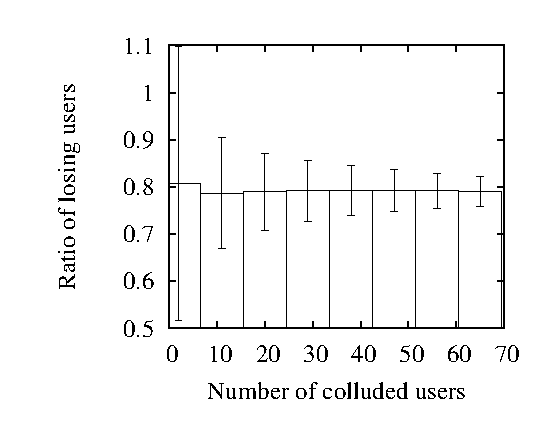
\includegraphics[width=\textwidth]{collusion_resist_codes/images/img_gs_ratio_con.eps}
%\caption{Ratios of losing colluded users for different collusion sizes in the continuous model.}
%\label{fig:gs_ratio_con}
%\end{minipage}
%\hspace{0.01cm}
%\begin{minipage}{0.24\textwidth}
%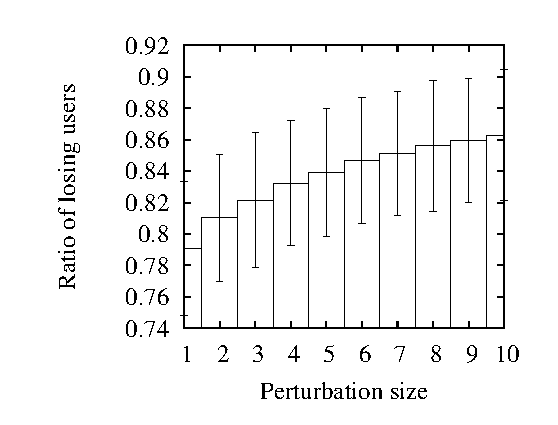
\includegraphics[width=\textwidth]{collusion_resist_codes/images/img_gs_perturb_con.eps}
%\caption{Ratios of losing colluded users for different strategy perturbation sizes in the continuous model.}
%\label{fig:gs_perturb_con}
%\end{minipage}
%\hspace{0.01cm}
%\begin{minipage}{0.24\textwidth}
%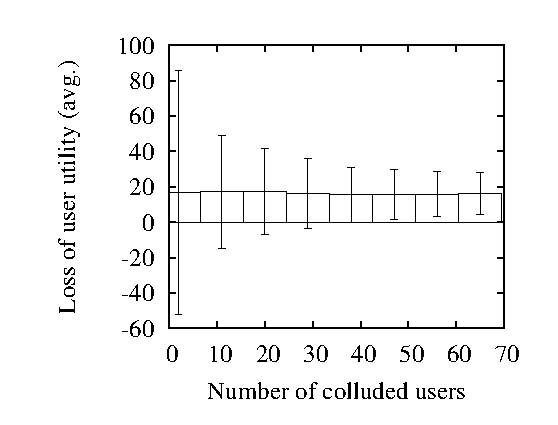
\includegraphics[width=\textwidth]{collusion_resist_codes/images/img_tr_loss_con.eps}
%\caption{Average loss on user utility for different collusion sizes in the continuous model.}
%\label{fig:tr_ratio_con}
%\end{minipage}
%\hspace{0.01cm}
%\begin{minipage}{0.24\textwidth}
%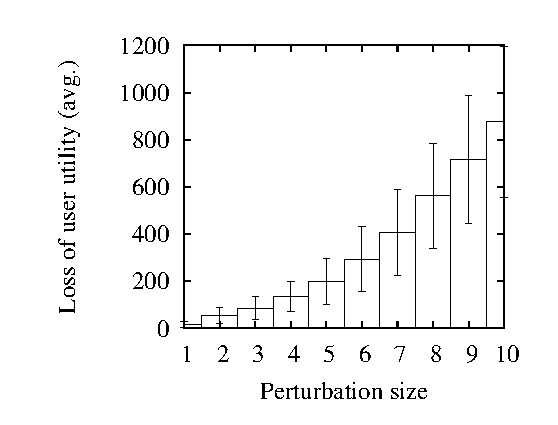
\includegraphics[width=\textwidth]{collusion_resist_codes/images/img_tr_perturb_con.eps}
%\caption{Average loss on user utility for different strategy perturbation sizes in the continuous model.}
%\label{fig:tr_perturb_con}
%\end{minipage}
%\end{figure*}
%
%A losing user is a colluded user who suffers utility loss when colluding. A perturbation $\varepsilon$ on user $i$'s truthful strategy $s_i = \kappa_i$ results in an untruthful strategy $s'_i = \kappa_i + \varepsilon$. Figure \ref{fig:gs_ratio_con} gives the fact that the ratio of losing users remains around 80\% for different numbers of colluded users. Its variation becomes more stable given more colluded users. Hence for any collusion, most colluded users may complain and quit. Figure \ref{fig:gs_perturb_con} shows that the ratio of losing users increases given more strategy perturbation. For any perturbation size larger than 1.0, more than 80\% colluded users may complaint about utility loss and thus quit the crowdsensing. This result verifies that if any user tries some strategies more deviant from the truthful costs, usually it will end in a larger utility loss. Thus Figure \ref{fig:gs_ratio_con} and Figure \ref{fig:gs_perturb_con} verify the results of group strategyproofness. Figure \ref{fig:tr_ratio_con} and Figure \ref{fig:tr_perturb_con} give the similar results on the average utility loss of the colluded users. That is, for different collusion sizes, each colluded user may suffer average utility loss of about 20. Average utility loss grows rapidly as the perturbation size increases. They verify that our continuous model achieves n-truthfulness.

\begin{figure*}[!t]
\centering
\begin{minipage}{0.3\textwidth}
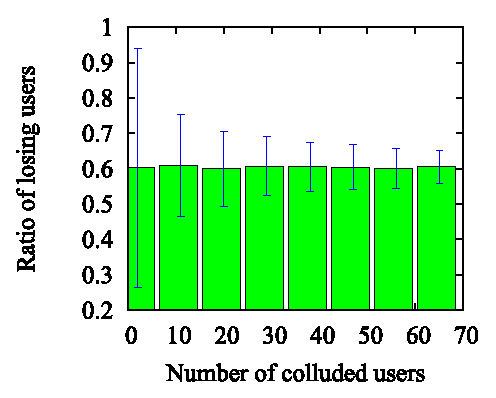
\includegraphics[width=\textwidth]{collusion_resist_codes/images/img_gs_ratio_dis.eps}
\caption{Ratios of losing colluded users for different collusion sizes.}
\label{fig:gs_ratio_dis}
\end{minipage}
\hspace{0.01cm}
\begin{minipage}{0.3\textwidth}
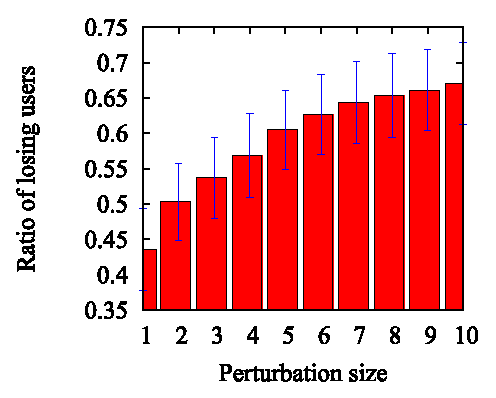
\includegraphics[width=\textwidth]{collusion_resist_codes/images/img_gs_perturb_dis.eps}
\caption{Ratios of losing colluded users for different strategy perturbation sizes.}
\label{fig:gs_perturb_dis}
\end{minipage}
\hspace{0.01cm}
\begin{minipage}{0.3\textwidth}
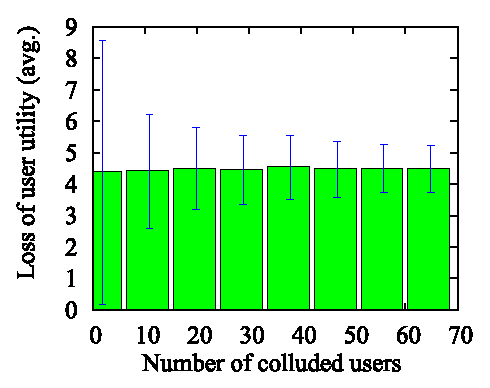
\includegraphics[width=\textwidth]{collusion_resist_codes/images/img_tr_loss_dis.eps}
\caption{Average loss on user utility for different collusion sizes.}
\label{fig:tr_ratio_dis}
\end{minipage}
\end{figure*}

\subsection{\color{black}Evaluation Results}
Based on Figure \ref{fig:gs_ratio_dis}, most colluded users (around 60\%) may complain the loss of their user utilities when in collusion. %The ratio is less than that of the continuous model (about 80\%), since some changed strategies are still bounded by the same partition, and as a result, they will result in the identical assigned task number and payment from the platform. 
Figure \ref{fig:gs_perturb_dis} shows the losing ratio increases given more perturbation size. For any perturbation size larger than 2.0, more than half of the colluded users will lose. By a similar reasoning, Figure \ref{fig:tr_ratio_dis} and Figure \ref{fig:tr_perturb_dis} show that any collusion may have negative impacts on the user utilities of the colluded users. For different collusion sizes, each colluded user may suffer average utility loss of more than 4. The perturbation size increasing by 1.0 will give utility loss of 1.0 to each colluded user averagely. Hence our simulation has verified that our {\color{black}incentive mechanism} is group strategyproof and n-truthful.

We also consider the platform utility. %In the continuous model, the platform utility is always $R$ for all collusion scenarios (see Section \ref{sec:opu}). Differently, 
Collusion has negative impacts on the platform utility. Figure \ref{fig:up_ratio_dis} shows that the platform utility suffers more loss given more colluded users. Figure \ref{fig:up_perturb_dis} reveals that the platform utility also suffers larger loss given more deviant perturbation on strategies. The underling reason is that each colluded user prefers to earn more payment by reporting low cost units. For example, if the collusion allows the user to report 0.01 or 2.00 as strategy, this user will prefer to report 0.01 rather than 2.00. As a result, when more users collude, or the perturbation size grows, the payment to each user can have more probability to increase rather than decrease. This will reduce the platform utility. On the other hand, collusion may give more variations on the platform utility. Thus by considering the utility, the platform expects to eliminate {\color{black}collusion among the users}.

\begin{figure*}[!t]
\centering
\begin{minipage}{0.3\textwidth}
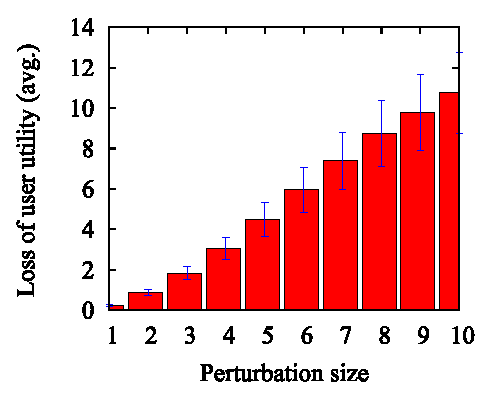
\includegraphics[width=\textwidth]{collusion_resist_codes/images/img_tr_perturb_dis.eps}
\caption{Average loss on user utility for different strategy perturbation sizes.}
\label{fig:tr_perturb_dis}
\end{minipage}
\hspace{0.01cm}
\begin{minipage}{0.3\textwidth}
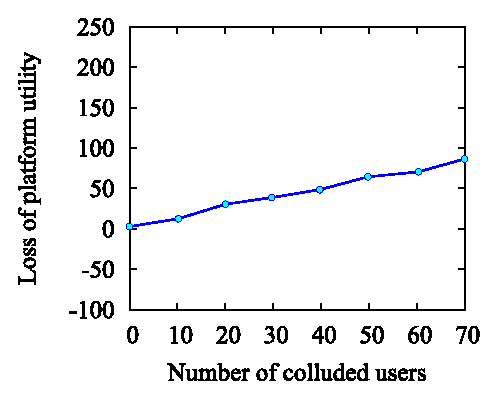
\includegraphics[width=\textwidth]{collusion_resist_codes/images/img_up_ratio_dis.eps}
\caption{Loss of platform utility for different collusion sizes.}
\label{fig:up_ratio_dis}
\end{minipage}
\hspace{0.01cm}
\begin{minipage}{0.3\textwidth}
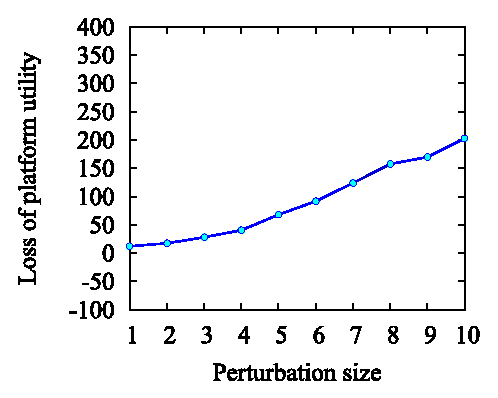
\includegraphics[width=\textwidth]{collusion_resist_codes/images/img_up_perturb_dis.eps}
\caption{Loss of platform utility for different strategy perturbation sizes.}
\label{fig:up_perturb_dis}
\end{minipage}
%\hspace{0.01cm}
%\begin{minipage}{0.24\textwidth}
%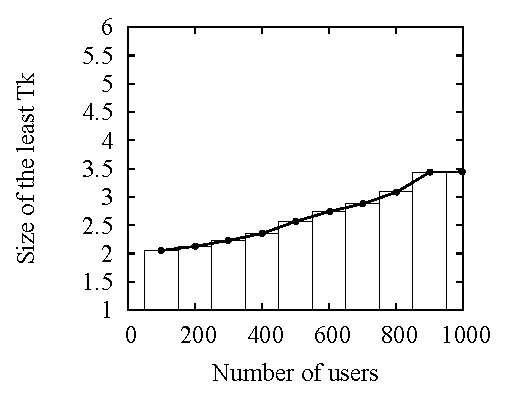
\includegraphics[width=\textwidth]{collusion_resist_codes/images/img_tk.eps}
%\caption{$\min |T_k|$ for different numbers of all users in the discrete model.}
%\label{fig:tk}
%\end{minipage}
%\hspace{0.01cm}
%\begin{minipage}{0.24\textwidth}
%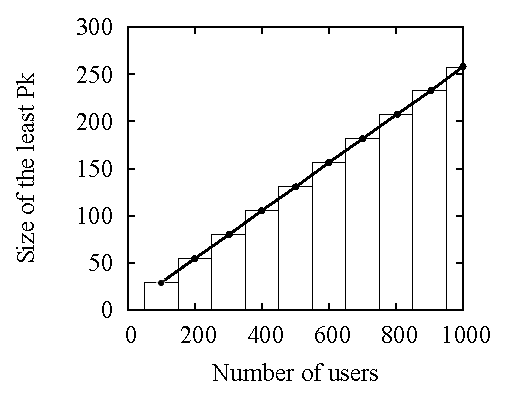
\includegraphics[width=\textwidth]{collusion_resist_codes/images/img_pk.eps}
%\caption{$\min |P_k|$ for different numbers of all users in the discrete model.}
%\label{fig:pk}
%\end{minipage}
\end{figure*}

%\subsection{Differential Privacy Evaluations}
%To ensure our differential privacy scheme can work, one expects large enough $\min |T_k|$ and $\min |P_k|$. Figure \ref{fig:tk} shows that each set $T_k$ has at least two users. In other words, there are always at least two users within any partition given by our algorithm. This is a direct consequence of merging partitions as proposed. Figure \ref{fig:pk} shows that for any partition, there are at least around one fourth of the total users whose cost unit range intervals intersect with this partition. Both facts can guarantee that any privacy leakage by too small $T_k$ and $P_k$ has very low possibility. For example, given 100 users, the least $P_k$ may have size of 25. The corresponding $|T_k|\geq 2$. Thus to identify all the users in $T_k$ takes probability less than $(1/25)^2 = 0.16\%$. Hence this fact ensures our mechanism can be 0-differentially private.

\section{Related Works}
\label{sec:rw}
Incentive mechanism design in crowdsensing applications has attracted a lot of attention in research \cite{ganti2011mobile, singer2013pricing, vukovic2010ubiquitous, yang2012crowdsourcing, zhao2012evaluation, koutsopoulos2013optimal, zhang2012reputation, singla2013truthful, jaimes2012location, singla2013incentives}. Among them the question how to make the participating users strategize truthfully has a lot of interests \cite{singer2013pricing, vukovic2010ubiquitous}. For example, Yang et al. \cite{yang2012crowdsourcing} proposed a truthful user-centric incentive mechanism for mobile phone crowdsensing. They used the truthful auction rule (Theorem 2.1 in \cite{singer2010budget}) to implement the computationally efficient mechanism in which each user had no incentive by lying about its cost. But the authors did not consider the scenario that the platform budget could be limited. To make the mechanism budget feasible, Singla et al. \cite{singla2013truthful} proposed another truthful incentive mechanism by making a few assumptions on each user's cost distribution. Similarly, Koutsopoulos \cite{koutsopoulos2013optimal} gave the closed form of truthful incentive payments for some continuous crowdsensing games by assuming each user's cost value is bounded within an interval. On the other hand, one may consider many other factors when designing incentive mechanisms for crowdsensing applications. Such factors include reputation mechanisms \cite{zhang2012reputation}, users' locations \cite{jaimes2012location}, privacy concerns \cite{singla2013incentives}, etc. Unfortunately, many of them could not achieve truthful mechanisms \cite{zhang2012reputation, jaimes2012location}.

Collusion attack on collaborative systems is also an important issue for research \cite{feng2013imac, chen2013sparc, zhong2007designing, zheng2014strategy}. Basically researchers give truthful incentive mechanisms by achieving strategyproof equilibria \cite{feng2013imac}. However, only strategyproofness cannot eliminate all the possible collusions among the users, since it is possible that a group of users know and trust each other completely, and thus they may safely change their strategies simultaneously to make their utilities higher than those given by equilibrium \cite{goldberg2005collusion, zhong2007designing}. To give a truthful incentive mechanism which is also resistant to any collusion, one may achieve group strategyproofness \cite{jain1999group, mas1995microeconomic} and t-truthful \cite{goldberg2005collusion,goldberg2003competitiveness}. Unfortunately, it is often impossible to find group strategyproofness or t-truthfulness for many cases. For instance, Zhong et al \cite{zhong2007designing} showed that group strategyproofness is impossible for many incentive-compatible routing games on ad hoc networks. Instead they achieved strong Nash equilibrium \cite{aumann1959acceptable, mas1995microeconomic}, another standard game theoretic solution, to defend against any collusion. The authors also leveraged some public key cryptographic techniques called restricted verifier signatures to eliminate profit trading. However, strong Nash equilibrium cannot guarantee truthfulness. On the other hand, since crowdsensing games are usually different from routing games in ad hoc networks\footnote{Usually one has to consider the graph model of network to reflect each participating user's task in routing games. However, we do not have to consider this graph model for most crowdsensing games.}, one cannot directly use routing incentive solutions to solve crowdsensing incentive problems. There are very few literatures on collusion resistance for crowdsensing applications. To the best of our knowledge, we are the first to investigate the possibility of group strategyproofness for crowdsensing incentive mechanisms.

\section{Conclusions}
\label{sec:con}
{\color{black}
This paper has systematically researched collusion attacks, including profit trading, in crowdsensing incentive mechanism. We have investigated the criteria that a truthful crowdsensing incentive mechanism can achieve group strategyproofness (eliminating collusion) or even n-truthfulness (eradicating profit trading). We have also proposed our crowdsensing incentive mechanism, which can resist any collusion attacks, even including profit trading. To verify our results, we have rigorously done the proofs that our solution can achieve the goals as stated above, and we have also given extensive simulations and presented all the supporting experimental results.
}

\bibliographystyle{./IEEEtran}
\bibliography{./13fall_1ed}
%\pagebreak

\appendix
{\color{black}
\subsection{Discussions on the Strategyproof Incentive Mechanism}
\label{sec:dsim}
In Section \ref{sec:PFSM} we have given the general incentive mechanism in which each user's private cost unit is unknown initially. To make each user report its own cost unit honestly, we need to find the forms of payment $p_i$ and sensing time $t_i$ that can achieve strategyproofness. In this section we discuss the closed-forms of payment and required sensing time for a strategyproof incentive mechanism.

We first analyze the required sensing time of each user. The major objective of our incentive mechanism is to make each user strategize truthfully ($s_i=\kappa_i$ always holds) if each user expects to maximize its own utility. This requirement restricts each user\rq{}s required sensing time $t_i(s_i)$\footnote{Here $t_i(s_i)$ denotes the required sensing time of user $i$ if its strategy is $s_i$, while other users\rq{} strategies are fixed. This paper always follows this notational convention.} to be non-increasing as the user strategy $s_i$ grows unilaterally. This restriction can be shown by the sum of the following inequalities:
\begin{equation}
\label{eqn:sum_ineq}
\begin{aligned}
&p_i(\kappa_i)-\kappa_it_i(\kappa_i)\geq p_i(\kappa_i')-\kappa_it_i(\kappa_i')\\
&p_i(\kappa_i')-\kappa_i't_i(\kappa_i')\geq p_i(\kappa_i)-\kappa_i't_i(\kappa_i)
\end{aligned}
\end{equation}
where $\kappa_i'>\kappa_i$. The first equation in (\ref{eqn:sum_ineq}) describes the case in which the cost unit of user $i$ is $\kappa_i$, and the second equation is when the cost unit is $\kappa_i'$. By summing both the equations in (\ref{eqn:sum_ineq}), one may verify the restriction $t_i(\kappa_i)\geq t_i(\kappa_i')$. We assume the required sensing time $t_i(s_i)$ is a non-increasing function from $\mathbb{R}^+$ to $\mathbb{R}^+$. Based on Theorem 7.8 in \cite{oxtoby1971measure}, $t_i(s_i)$ is differentiable a.e. (almost everywhere). Thus, we have $\frac{\partial t_i}{\partial s_i}\leq 0$ a.e. holds.

We next analyze the payment to each user. For the truthfulness, the utility $u_i$ of each user $i$ maximizes at its real cost unit $\kappa_i$ whatever strategies other users take. Based on (\ref{eqn:user_utility_2}), we have
\begin{equation}
\label{eqn:drv_u}
\frac{\partial u_i}{\partial s_i}(\kappa_i) = \frac{\partial p_i}{\partial s_i}(\kappa_i)-\kappa_i \frac{\partial t_i}{\partial s_i}(\kappa_i)=0
\end{equation}
holds for any $\kappa_i\in\mathbb{R}^+$. Usually, for each user, the more cost unit it will suffer, the more reluctant it will be to participate in crowdsensing. If the user would like to be out of the crowdsensing game, it just declares a very large cost unit. As a result, its utility should be 0 in nature. Thus, it is reasonable to assume both the payment $p_i$ and the required sensing time $t_i$ will finally converge to 0: $\lim_{s_i\to+\infty}p_i(s_i)=0$, $\lim_{s_i\to+\infty}t_i(s_i)=0$. Based on this boundary condition and (\ref{eqn:drv_u}), we have\footnote{Here we replace $s_i$ by $s$ to avoid notational confusion.}
\begin{equation}
\int_{s_i}^{+\infty}\frac{\mathrm{d} u_i}{\mathrm{d} s}(s) \mathrm{d}s
=-p_i(s_i)+s_it_i(s_i)+\int_{s_i}^{+\infty}t_i(s)\mathrm{d}s=0,
\end{equation}
which gives the closed-form of $p_i(s_i)$\footnote{Here we choose proper $t_i(s)$ to make the integral $\int_{s_i}^{+\infty}t_i(s)\mathrm{d}s$ converge.}
\begin{equation}
\label{eqn:payment}
p_i(s_i)=s_it_i(s_i)+\int_{s_i}^{+\infty}t_i(s)\mathrm{d}s.
\end{equation}
Thus, the utility of user $i$ is
\begin{equation}
\label{eqn:utility_final}
u_i(s_i)=(s_i-\kappa_i)t_i(s_i)+\int_{s_i}^{+\infty}t_i(s)\mathrm{d}s.
\end{equation}
We discuss the payment $p_i$ and the user utility $u_i$ here in an intuitive way. Figure \ref{fig:truthful_payment} illustrates the geometric relation between payment and user utility. Clearly user utility maximizes at the value $s_i = \kappa_i$ exactly, and the maximum user utility is the area of $ABC$.
\begin{figure}[!t]
\centering{}
\setlength{\unitlength}{1cm}
\begin{picture}(4.0,4.2)(-2.0,-0.5)
\put (-4,0){\vector(1,0){7.5}}% draw x axe
\put (-4,0){\vector(0,1){3.8}} %draw y axe
\put (-4,3.9){$t_i$}
% give the t curve
\qbezier (-4,3.5)(-2,2)(3.5,0.1)
% give strategy \kappa_i
\put (-1.5,-0.3){$\kappa_i$}
\multiput (-1.5,0)(0,0.2){15}{\line (0,1){0.1}}
\put (-3.1,-0.3){$s_2$}
\multiput (-3.1,0)(0,0.2){15}{\line (0,1){0.1}}
\multiput (-3.0,2.9)(0.2,0){8}{\line (1,0){0.1}}
\put (1.3,-0.3){$s_1$}
\multiput (1.3,0)(0,0.2){5}{\line (0,1){0.1}}
\multiput (-1.4,0.9)(0.2,0){14}{\line (1,0){0.1}}
\put (3.0,-0.3){$s_i$}
% give labels
\put (-4.2,-0.3){$O$}
\put (3.7,-0.1){$B$ $+\infty$}
\put (-1.4, 2.1){$A$}
\put (-1.8, 0.1){$C$}
\put (-1.8, 0.9){$D$}
\put (1.4, 0.9){$E$}
\put (-3.2, 3){$F$}
\put (-1.4, 3){$G$}
\end{picture}
\caption{The relation between user strategy $s_i$ and user utility $u_i$ in the strategyproof crowdsensing incentive mechanism. Here $s_1 > \kappa_i > s_2$. For $s_1$, we have $u_i(s_1)$ is equal to the area of $DEBC$. For $s_2$, we have $u_i(s_2)$ is equal to the area of $ABC$ minus the area of $AFG$. Obviously the area of user utility maximizes at the value $s_i = \kappa_i$.}
\label{fig:truthful_payment}
\end{figure}

We next analyze the user utility obtained by the above truthful mechanism. For each user $i$\rq{}s own strategy $s_i$, we have
\begin{equation}
\frac{\partial u_i}{\partial s_i}=(s_i-\kappa_i)\frac{\partial t_i}{\partial s_i}.
\end{equation}
It is easy to verify $\frac{\partial u_i}{\partial s_i}(\kappa_i)=0$. {\color{black}To be truthful, we have $\frac{\partial t_i}{\partial s_i}(s_i)\leq 0$ a.e. holds. Thus $\frac{\partial u_i}{\partial s_i}\leq 0$ a.e. for $s_i>\kappa_i$, and $\frac{\partial u_i}{\partial s_i}\geq 0$ a.e. for $s_i<\kappa_i$. Since $u_i$ can be established by the following Lebesgue integration:
\begin{equation}
\label{eqn:lebes}
u_i(s_i) = u_i(\kappa_i) + \int_{\kappa_i}^{s_i}\frac{\partial u_i}{\partial s_i}(s)\mathrm{d}s.
\end{equation} 
Clearly $u_i(\kappa_i)\geq u_i(s_i)$ for any $s_i\in \mathbb{R}^+$. But the uniqueness of maximum points of $u_i$ needs further discussion. 
If $\kappa_i$ is a condensation point\footnote{Every open interval (neighborhood) including the condensation point must have \emph{uncountably infinite} points in the given set. Assuming Continuum Hypothesis, the intersection of every open neighborhood and the given set must contain some open interval.} of some open interval $I$ s.t. for any $s_i\in I$, $\frac{\partial t_i}{\partial s_i}(s_i)=0$, then (\ref{eqn:lebes}) shows that every point in $I$ maximizes $u_i$. Our discrete crowdsensing model is one instance of this scenario. Otherwise, $s_i=\kappa_i$ is the \emph{unique} solution to maximize $u_i$, since $\kappa_i$ is within some open interval $E$, in which $\frac{\partial t_i}{\partial s_i}(s_i)<0$ a.e. holds. Suppose for any $s_i>\kappa_i$, we have
\begin{equation}
\begin{aligned}
u_i(s_i) &= u_i(\kappa_i) + \left\{\int_{(\kappa_i,s_i)\cap E} + \int_{(\kappa_i,s_i)\setminus E} \right\} \frac{\partial u_i}{\partial s_i}(s)\mathrm{d}s \\
&\leq u_i(\kappa_i) + \int_{(\kappa_i,s_i)\cap E}\frac{\partial u_i}{\partial s_i}(s)\mathrm{d}s < u_i(\kappa_i).\\
\end{aligned}
\end{equation}
The case for any $s_i<\kappa_i$ is analogous.
} 

For any other user strategy $s_j$, we have
\begin{equation}
\label{eqn:p_ui_j}
\frac{\partial u_i}{\partial s_j}(\kappa_i,s_j)=\int_{\kappa_i}^{+\infty}\frac{\partial t_i}{\partial s_j}(s,s_j)\mathrm{d}s.
\end{equation}
We are not sure whether $\frac{\partial u_i}{\partial s_j}(\kappa_i,s_j)=0$ based on (\ref{eqn:p_ui_j}). Since we have no knowledge of $\kappa_i$ when we design the closed-form of $t_i(s_i)$, in order to assume $\frac{\partial u_i}{\partial s_j}(\kappa_i,s_j)\not=0$, we must guarantee $\int_{s_i}^{+\infty}\frac{\partial t_i}{\partial s_j}(s,s_j)\mathrm{d}s\not=0$ holds for any $s_i\in\mathbb{R}^+$.\footnote{Similarly, we must guarantee $\int_{s_i}^{+\infty}\frac{\partial t_i}{\partial s_j}(s,s_j)\mathrm{d}s=0$ holds for any $s_i\in\mathbb{R}^+$ to ensure $\frac{\partial u_i}{\partial s_j}(\kappa_i,s_j)=0$, which is the opposite case of Definition \ref{def:pd}. That is, we avoid the case $\int_{s_i}^{+\infty}\frac{\partial t_i}{\partial s_j}(s,s_j)\mathrm{d}s=0$ holds partially over $\mathbb{R}^+$ when designing the function $t_i$ for this paper.} Insightfully, this reveals the \emph{dependency} between the function value $u_i(s_i,s_j)$ and the parameter $s_j$. That is, the strategy $s_j$ contributes significantly to the utility of user $i$. Thus, we introduce the concept of \emph{parametric dependency}.
\begin{definition}
\label{def:pd}
\textbf{(Parametric Dependency)} The utility function $u_i(s_i,s_j)=p_i(s_i,s_j)-\kappa_it_i(s_i,s_j)$ is parametric dependent on $s_j$ if and only if $\int_{s_i}^{+\infty}\frac{\partial t_i}{\partial s_j}(s,s_j)\mathrm{d}s\not=0$ holds for any $s_i\in\mathbb{R}^+$.
\end{definition}
For example, let $t_i(s_i,s_j)=s_j\mathrm{e}^{-s_i}$, and thus $\frac{\partial t_i}{\partial s_j}(s_i,s_j)=\mathrm{e}^{-s_i}>0$. Then we have $\int_{s_i}^{+\infty}\frac{\partial t_i}{\partial s_j}(s,s_j)\mathrm{d}s>0$ and thus $u_i(s_i,s_j)$ is parametric dependent on $s_j$. In fact, when $s_i=\kappa_i$, $\frac{\partial u}{\partial s_j}(\kappa_i,s_j)=\int_{\kappa_i}^{+\infty}\frac{\partial t_i}{\partial s_j}(s,s_j)\mathrm{d}s>0$. That is, the utility of user $i$ will increase as user $j$\rq{}s strategy increases around the maximum points. Similarly, it can derive that $u_i(s_i,s_j)$ is not parametric dependent on any $s_k$ such that $k\not=i,j$. If $u_i$ is not parametric dependent on $s_j$, $s_j$ has no impact on $u_i$, and thus user $i$ can maximize its utility by choosing truthful strategy, whatever $s_j$ is. This is because for any different strategies $s_j$ and $s'_j$, we have
\begin{equation}
\label{eqn:unpd}
u_i(s_j)=u_i(s'_j)+\int_{s'_j}^{s_j}\frac{\partial u_i}{\partial s_j}(s)\mathrm{d}s=u_i(s'_j),
\end{equation}
in which $\frac{\partial u_i}{\partial s_j}=0$ always holds.
}
\subsection{Local Properties of Bivariate Functions}
This paper leverages the local properties of the bivariate functions (i.e., the user utility functions) at the maximum points of the slices. A differentiable bivariate function $u(x,y)$ maps $\mathbb{R}^2$ to $\mathbb{R}$, and we can obtain a slice function $u(x,y_0)$ by fixing $y=y_0$. We assume there exists a point $(x_0,y_0)$ such that $\frac{\partial u}{\partial x}(x_0,y_0)=0$ and $\frac{\partial^2 u}{\partial x^2}(x_0,y_0)<0$. That is, the slice function $u(x,y_0)$ is \emph{concave} over the neighborhood of $(x_0,y_0)$. However, for the other variable $y$ we assume $\frac{\partial u}{\partial y}(x_0,y_0)\not=0$. That is, the slice function $u(x_0,y)$ is either increasing or decreasing over the neighborhood of $(x_0,y_0)$. Then there is a boundary distinguishing the areas $\{(x,y)|u(x,y)<u(x_0,y_0)\}$ and $\{(x,y)|u(x,y)>u(x_0,y_0)\}$, and each point $(x,y)$ on the boundary satisfies $u(x,y)=u(x_0,y_0)$ (see Figure \ref{fig:local_bivariate}). Over the neighborhood of $(x_0,y_0)$, the boundary curve $\{(x,y)|u(x,y)=u(x_0,y_0)\}$ satisfies
\begin{equation}
\frac{\partial u}{\partial x}(x_0,y_0)+\frac{\partial u}{\partial y}(x_0,y_0)\frac{\mathrm{d} y}{\mathrm{d} x}\bigg|_{y=y_0}=0.
\end{equation}
Since $\frac{\partial u}{\partial x}(x_0,y_0)=0$ and $\frac{\partial u}{\partial y}(x_0,y_0)\not=0$, we have $\frac{\mathrm{d} y}{\mathrm{d} x} = 0$ at $(x_0,y_0)$. That is, for any positive number $\varepsilon>0$, we have $\delta>0$ such that for any $0<|x-x_0|<\delta$, $|\frac{y-y_0}{x-x_0}|<\varepsilon$ holds. We may assume $\varepsilon=1$, and then there exists $\delta>0$ such that $|y-y_0|<|x-x_0|$ for any $0<|x-x_0|<\delta$. Thus for any point $(x,y)$ satisfies $|y-y_0|=|x-x_0|$ and $0<|x-x_0|<\delta$, we have $u(x,y)\not=u(x_0,y_0)$. If $\frac{\partial u}{\partial y}(x_0,y_0)>0$, for any point $(x,y)$ satisfies $y-y_0=|x-x_0|,0<|x-x_0|<\delta$, we have $u(x,y)>u(x_0,y_0)$. Similarly, if $\frac{\partial u}{\partial y}(x_0,y_0)<0$, for any point $(x,y)$ satisfies $y_0-y=|x-x_0|,0<|x-x_0|<\delta$, we have $u(x,y)>u(x_0,y_0)$. That is, we can always find uncountably infinite points in the neighborhood of $(x_0,y_0)$ to increase the function value $u(x,y)$ and make it larger than $u(x_0, y_0)$. We summarize the above discussions as Lemma \ref{lem:bf}.
\begin{lemma}
\label{lem:bf}
For any bivariate function $u(x,y)$ such that $\frac{\partial u}{\partial x}(x_0,y_0)=0$ at point $(x_0,y_0)$, 
\begin{enumerate}
\item if $\frac{\partial u}{\partial y}(x_0,y_0)>0$, there exists $\delta>0$ such that for any point $(x,y)$ satisfies $y-y_0=|x-x_0|,0<|x-x_0|<\delta$, we have $u(x,y)>u(x_0,y_0)$;
\item if $\frac{\partial u}{\partial y}(x_0,y_0)<0$, there exists $\delta>0$ such that for any point $(x,y)$ satisfies $y_0-y=|x-x_0|,0<|x-x_0|<\delta$, we have $u(x,y)>u(x_0,y_0)$.
\end{enumerate}
\end{lemma}

\begin{figure}[!t]
\centering{}
\setlength{\unitlength}{1cm}
\begin{picture}(4,4)(-1.5,-0.5)
\put (-0.5,-0.4){$(x_0,y_0)$}% draw the original point label
\put (-2.5,0){\vector(1,0){5.0}}% draw x axe
\put (2.75,-0.05){$x$}
\put (0,0){\vector(0,1){3.2}} %draw y axe
\put (0,3.35){$y$}
\qbezier(0,0)(-1.25,0)(-2.5,2.8)% draw graph
\qbezier(0,0)(1.25,0)(2.5,2.8)
\put (-1.2,1.5){$u(x,y)>u(x_0,y_0)$}
\put (2,0.6){$u(x,y)<u(x_0,y_0)$}
\put (2,3){$u(x,y)=u(x_0,y_0)$}
\put (2.1,1.5){$\frac{\partial u}{\partial y}(x_0,y_0)>0$}
\put (2.8,2.8){\vector(-1,0){0.3}}
\put (0,0){\vector(1,1){1}}
\put (0,0){\vector(-1,1){1}}
\multiput (1,1)(0,-0.1){10}{\line(0,-1){0.05}}
\multiput (-1,1)(0,-0.1){10}{\line(0,-1){0.05}}
\put (0.9,-0.4){$x_0+\delta$}
\put (-1.8,-0.4){$x_0-\delta$}
\end{picture}
\caption{Local scenario of bivariate function at maximum point of its slice.}
\label{fig:local_bivariate}
\end{figure}

\end{document}